%%%%%%%%%%%%%%%%%%%%%%%%%%%%%%%%%%%%%%%%%%%%%%%%%%%
%% LaTeX book template                           %%
%% Author:  Amber Jain (http://amberj.devio.us/) %%
%% License: ISC license                          %%
%%%%%%%%%%%%%%%%%%%%%%%%%%%%%%%%%%%%%%%%%%%%%%%%%%%
\documentclass[12pt]{book}
%\documentclass[a4paper,12pt]{book}
\usepackage{iftex}
\ifPDFTeX
  % PDFLaTeX or LaTeX 
  \usepackage[utf8]{inputenc}
  \usepackage[T1]{fontenc}
  \DeclareUnicodeCharacter{00B5}{\ensuremath{\mu}}
\else
  %  XeLaTeX or LuaLaTeX
  \usepackage{fontspec}
\fi
\usepackage[left=2cm,right=1cm,top=2cm,bottom=2cm,headheight=1cm]{geometry}

\usepackage{lmodern}
\usepackage{amsmath}
\usepackage{textcomp}
\usepackage{multicol}
\usepackage[]{ragged2e}
\usepackage[dvipsnames]{xcolor}
\usepackage{blindtext}
%%%%%
\usepackage[12pt]{moresize}
%\fontsize{8}{20}\selectfont
\usepackage{amssymb}
\usepackage{enumerate}
%%%%%
\usepackage{pifont}
\usepackage{braket}
\usepackage{esint}
\usepackage{ziffer}
\usepackage{latexsym}
\usepackage[normalem]{ulem}
\usepackage{color,tikz}
\usepackage{mathtools}
\usepackage{setspace}
\usepackage{tocloft}
\usepackage{longtable}
\usepackage{url}
\usepackage{booktabs}
\usepackage{float}
\usepackage{graphicx, nicefrac}
\usepackage{scalefnt}
\usepackage{tikz}
\usepackage[sans]{dsfont}
\usetikzlibrary{decorations.pathmorphing}
\usetikzlibrary{shapes.geometric, arrows}
\usepackage[ruled, vlined, linesnumbered]{algorithm}
\usepackage{caption}%
\usepackage[Sonny]{fncychap}
\usepackage[weather, clock]{ifsym}
\usepackage[most]{tcolorbox}
%%%%%%%%%%%%%%%%%%%%%%%%%%%%%%%%%%%%%%%%%%%%%%%%%%%%%%%%%
% Configurações para o Maxima %
%%%%%%%%%%%%%%%%%%%%%%%%%%%%%%%%%%%%%%%%%%%%%%%%%%%%%%%%%
%\usepackage{mathastext}
\usepackage{grffile}
\usepackage{ifthen}
\newsavebox{\picturebox}
\newlength{\pictureboxwidth}
\newlength{\pictureboxheight}
\newcommand{\includeimage}[1]{
    \savebox{\picturebox}{\includegraphics{#1}}
    \settoheight{\pictureboxheight}{\usebox{\picturebox}}
    \settowidth{\pictureboxwidth}{\usebox{\picturebox}}
    \ifthenelse{\lengthtest{\pictureboxwidth > .95\linewidth}}
    {
        \includegraphics[width=.95\linewidth,height=.80\textheight,keepaspectratio]{#1}
    }
    {
        \ifthenelse{\lengthtest{\pictureboxheight>.80\textheight}}
        {
            \includegraphics[width=.95\linewidth,height=.80\textheight,keepaspectratio]{#1}
            
        }
        {
            \includegraphics{#1}
        }
    }
}
\newlength{\thislabelwidth}
\DeclareMathOperator{\abs}{abs}

\definecolor{labelcolor}{RGB}{100,0,0}
\usepackage{physics}
%%%%%%%%%%%%%%%%%%%%%%%%%%%%%%%%%%%%%%%%%%%%%%%%%%%%%%%%%
% Source: http://en.wikibooks.org/wiki/LaTeX/Hyperlinks %
%%%%%%%%%%%%%%%%%%%%%%%%%%%%%%%%%%%%%%%%%%%%%%%%%%%%%%%%%
\usepackage{hyperref}
%\usepackage{graphicx}
\usepackage[portuguese]{babel}

%%%%%%%%%%%%%%%%%%%%%%%%%%%%%%%%%%%%%%%%%%%%%%%%%%%%%%%%%%%%%%%%%%%%%%%%%%%%%%%%
% 'dedication' environment: To add a dedication paragraph at the start of book %
% Source: http://www.tug.org/pipermail/texhax/2010-June/015184.html            %
%%%%%%%%%%%%%%%%%%%%%%%%%%%%%%%%%%%%%%%%%%%%%%%%%%%%%%%%%%%%%%%%%%%%%%%%%%%%%%%%
\newenvironment{dedication}
{
   \cleardoublepage
   \thispagestyle{empty}
   \vspace*{\stretch{1}}
   \hfill
   \begin{minipage}[t]{0.66\textwidth}
   \raggedright
}
{
   \end{minipage}
   \vspace*{\stretch{3}}
   \clearpage
}

%%%%%%%%%%%%%%%%%%%%%%%%%%%%%%%%%%%%%%%%%%%%%%%%
% Chapter quote at the start of chapter        %
% Source: http://tex.stackexchange.com/a/53380 %
%%%%%%%%%%%%%%%%%%%%%%%%%%%%%%%%%%%%%%%%%%%%%%%%
\makeatletter
\renewcommand{\@chapapp}{}% Not necessary...
\newenvironment{chapquote}[2][2em]
  {\setlength{\@tempdima}{#1}%
   \def\chapquote@author{#2}%
   \parshape 1 \@tempdima \dimexpr\textwidth-2\@tempdima\relax%
   \itshape}
  {\par\normalfont\hfill--\ \chapquote@author\hspace*{\@tempdima}\par\bigskip}
\makeatother

%%%%%%%%%%%%%%%%%%%%%%%%%%%%%%%%%%%%%%%%%%%%%%%%%%%
% First page of book which contains 'stuff' like: %
%  - Book title, subtitle                         %
%  - Book author name                             %
%%%%%%%%%%%%%%%%%%%%%%%%%%%%%%%%%%%%%%%%%%%%%%%%%%%

% Book's title and subtitle
\title{\Huge \textbf{\MakeUppercase{Simulações de Ondulatória com Uso do Maxima}} \footnote{This is a footnote.} \\  }
% Author
\author{\textsc{Elielzer Nuayed}\thanks{\url{https://github.com/elielzer}}}


\begin{document}
\frontmatter
\maketitle

%%%%%%%%%%%%%%%%%%%%%%%%%%%%%%%%%%%%%%%%%%%%%%%%%%%%%%%%%%%%%%%
% Add a dedication paragraph to dedicate your book to someone %
%%%%%%%%%%%%%%%%%%%%%%%%%%%%%%%%%%%%%%%%%%%%%%%%%%%%%%%%%%%%%%%
\begin{dedication}
Dedicated to Calvin and Hobbes.
\end{dedication}

%%%%%%%%%%%%%%%%%%%%%%%%%%%%%%%%%%%%%%%%%%%%%%%%%%%%%%%%%%%%%%%%%%%%%%%%
% Auto-generated table of contents, list of figures and list of tables %
%%%%%%%%%%%%%%%%%%%%%%%%%%%%%%%%%%%%%%%%%%%%%%%%%%%%%%%%%%%%%%%%%%%%%%%%
{\tableofcontents}
{\listoffigures}
{\listoftables}

\mainmatter

%%%%%%%%%%%
% Preface %
%%%%%%%%%%%
\chapter*{Preface}
Este livro foi concebido a partir de um \emph{insight} pessoal após eu ler um anúncio sobre uso do \emph{Maxima} no ensino da Física. Então veio-me a ideia de escrever algo nesse sentido.
Escolhi sobre ondulatória. O Maxima é introduzido no contexto como ambiente de apoio no momento que seja necessário simular as proposições. Dentre as proposições abordaremos situações clássicas, pois o objetivo é justamente apresentar o cartel de ferramentas desse software adequadas para transcrever a linguagem da física para representar as situações problema.



%%%%%%%%%%%%%%%%
% NEW CHAPTER! %
%%%%%%%%%%%%%%%%
\chapter{INTRODUÇÃO}
\begin{chapquote}{Author's name, \textit{Source of this quote}}
``This is a quote and I don't know who said this.''
\end{chapquote}
\section{Sobre o Maxima}
De acordo com descrição no site fabricante, o Maxima é um programa de computador do tipo multiplataforma, ou seja, ele está preparado para trabalhar (compilar) sob diversos sistemas operacionais ou plataformas computacionais.
Ainda de acordo com esse site o Maxima é uma versão evoluída de software especialista Macsyma. Os sistemas especialistas foram criados com a finalidade de reproduzir o raciocínio ou expertise de um  profissional de alguma área de conhecimento específica.

Assm,o Maxima é um sistema especialista para a manipulação de expressões matemáticas, tanto na forma simbólica como na forma numérica, incluindo:
\begin{itemize}
    \item diferenciação,
    \item integração,
    \item séries de Taylor,
    \item transformadas de Laplace,
    \item equações diferenciais ordinárias,
    \item sistemas de equações lineares,
    \item polinômios,
    \item conjuntos,
    \item listas,
    \item vetores,
    \item matrizes e
    \item tensores.
\end{itemize}

\noindent O que caracteriza a matemática simbólica é de não estar atrelada a um determinado idioma, por exemplo a expressão algébrica: \(x+2=7\), tem o mesmo significado em qualquer idioma. Portanto o Maxima é um sistema algébrico computacional para auxílio no cálculo e manipulação da  matemática simbólica visado simplificar o esforço de trabalho do estudante ou profissional (professor ou pesquisador).

O Maxima produz também resultados numéricos de alta precisão usando frações exatas, inteiros de precisão arbitrária e números de ponto flutuante de precisão variável. O Maxima pode plotar funções e dados em duas e três dimensões. Utilizaremos em nossos desenvolvimentos a plataforma gráfica do wxMaxima\textregistered .

%%%%%%%%%%%%%%%%%%%%%%%%%%%%%%%%%%%%%%%%%%%%%%%%%%%%%%%
% Sample table                                        %
% Source: www1.maths.leeds.ac.uk/latex/TableHelp1.pdf %
%%%%%%%%%%%%%%%%%%%%%%%%%%%%%%%%%%%%%%%%%%%%%%%%%%%%%%%
\begin{table}[ht]
\caption{Sample table} % title of Table
\centering % used for centering table
\begin{tabular}{c c c c}
% centered columns (4 columns)
\hline\hline %inserts double horizontal lines
S. No. & Column\#1 & Column\#2 & Column\#3 \\ [0.5ex]
% inserts table
%heading
\hline % inserts single horizontal line
1 & 50 & 837 & 970 \\
2 & 47 & 877 & 230 \\
3 & 31 & 25 & 415 \\
4 & 35 & 144 & 2356 \\
5 & 45 & 300 & 556 \\ [1ex] % [1ex] adds vertical space
\hline %inserts single line
\end{tabular}
\label{table:nonlin} % is used to refer this table in the text
\end{table}
\section{Como Instalar o wxMaxima\textregistered}
Instalar um software é uma tarefa que a maioria de usuários de PC já fizeram alguma vez, e instalar o Maxima é uma tarefa que não haverá muita dificuldade. O primeiro passo é obter o arquivo instalador. Uma opção é fazer o processo de \emph{download} do endereço da internet ou URL (sugestão do autor): maxima.sourceforge.io/windows-install.html (\ref{fig:site-maxima}). 
\begin{figure}[htbp!]
    \centering
    \caption{Entrando com a URL, para buscar a página do Maxima no \emph{Google}.}
        \label{fig:site-maxima}
    %\begin{Center}
    
\includegraphics[]{site-maxima.jpg}
	%\end{Center}
\end{figure}
\noindent A página na figura \ref{fig:pagina-maxima} contém um passo a passo, que é recomendável que seja lido. Entretando, por ora seguiremos mais focados no processo operacional de instalação em si. 
Assim, localize o link, nessa página com o texto: \href{sourceforge.net/projects/maxima/files/Maxima-Windows/5.46.0-Windows/}{5.46.0-Windows}, como mostrado nessa imagem.

\begin{figure}[htbp!]
    \centering
    \caption{Página encontrada do Maxima no navegador da Internet.}
        \label{fig:pagina-maxima}
    %\begin{Center}
    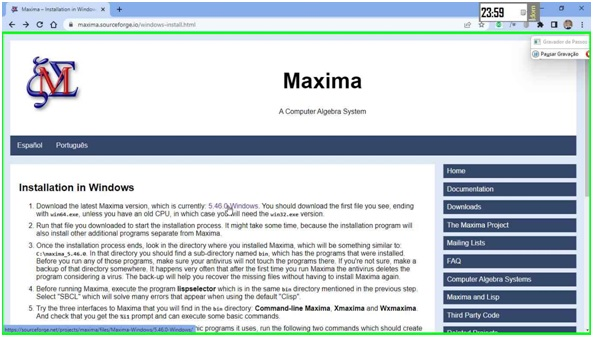
\includegraphics[]{pagina-maxima.jpg}
	%\end{Center}	
\end{figure}
\newpage
\noindent	Como forma de gerenciar o processo de instalação são apresentadas a seguir as janelas que interagem nas diversa etapas dessa instalação.
\begin{figure}[htbp!]
    \centering
    \caption{Janela que apresenta o início do processo de instalação.}
        \label{fig:maxima-ist-1}
    %\begin{Center}
    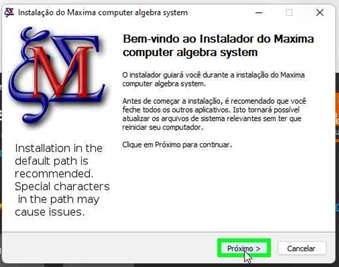
\includegraphics[]{maxima-ist-1.jpg}
	%\end{Center}
\end{figure}

	\begin{figure}[htbp!]
    \centering
    \caption{Janela que apresenta os termos de uso.}
        \label{fig:maxima-ist-2}
    %\begin{Center}
    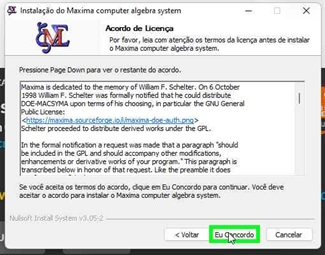
\includegraphics[]{maxima-ist-2.jpg}
	%\end{Center}
\end{figure}

	\begin{figure}[htbp!]
    \centering
    \caption{Janela que apresenta o diretório local para instalação de arquivos.}
        \label{fig:maxima-ist-3}
    %\begin{Center}
    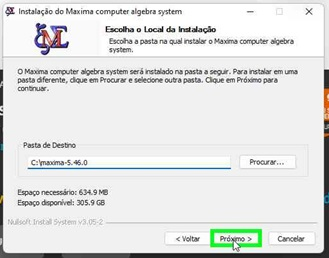
\includegraphics[]{maxima-ist-3.jpg}
	%\end{Center}
\end{figure}

	\begin{figure}[htbp!]
    \centering
    \caption{Janela de configuração de atalhos.}
        \label{fig:maxima-ist-4}
    %\begin{Center}
    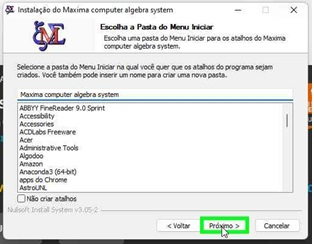
\includegraphics[]{maxima-ist-4.jpg}
	%\end{Center}
\end{figure}

	\begin{figure}[htbp!]
    \centering
    \caption{Janela de configuração do escopo de funções do programa.}
        \label{fig:maxima-ist-5}
    %\begin{Center}
    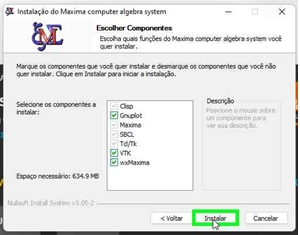
\includegraphics[]{maxima-ist-5.jpg}
	%\end{Center}
\end{figure}

	\begin{figure}[htbp!]
    \centering
    \caption{Janela de status do processo de instalação.}
        \label{fig:maxima-ist-6}
    %\begin{Center}
    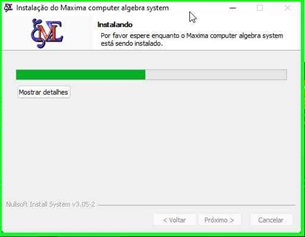
\includegraphics[]{maxima-ist-6.jpg}
	%\end{Center}
\end{figure}

	\begin{figure}[htbp!]
    \centering
    \caption{Janela de confirmação da instalação.}
        \label{fig:maxima-ist-7}
    %\begin{Center}
    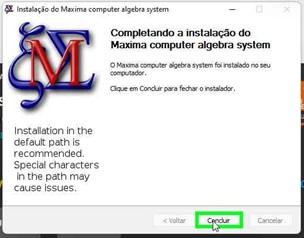
\includegraphics[]{maxima-ist-7.jpg}
	%\end{Center}
\end{figure}

	\begin{figure}[htbp!]
    \centering
    \caption{Aspecto do comando de menu na janela inicial do Windows.}
        \label{fig:menu-windows}
    %\begin{Center}
    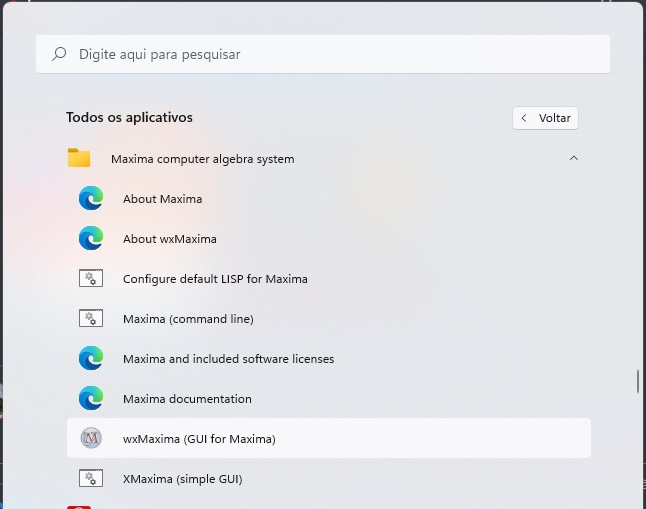
\includegraphics[scale=0.7]{menu-windows.jpg}
	%\end{Center}
\end{figure}
\newpage
\section{Conhecendo a \emph{Interface} Gráfica do wxMaxima}
A janela do aplicativo Maxima é idêntica a um editor de texto, e permite criar um arquivo, abrir um existente e salvar suas alterações, tudo a partir de um um menu supenso de comandos. Ao abrir a janela do aplicativo, esta já fornece de imediato, um prompt para a entrada de comandos de programação, ou textos descritivos, figura \ref{fig:tela-inicial}. A janela do aplicativo Maxima é idêntica a um editor de texto, porém sua funcionalidade lógica é identica á de uma planilha de cálculo, ou seja as janela possui uma estrutura baseada em células de cálculo.

	\begin{figure}[h]
    \centering
    \caption{Aspecto da janela do aplicativo Maxima.}
        \label{fig:tela-inicial}
    %\begin{Center}
    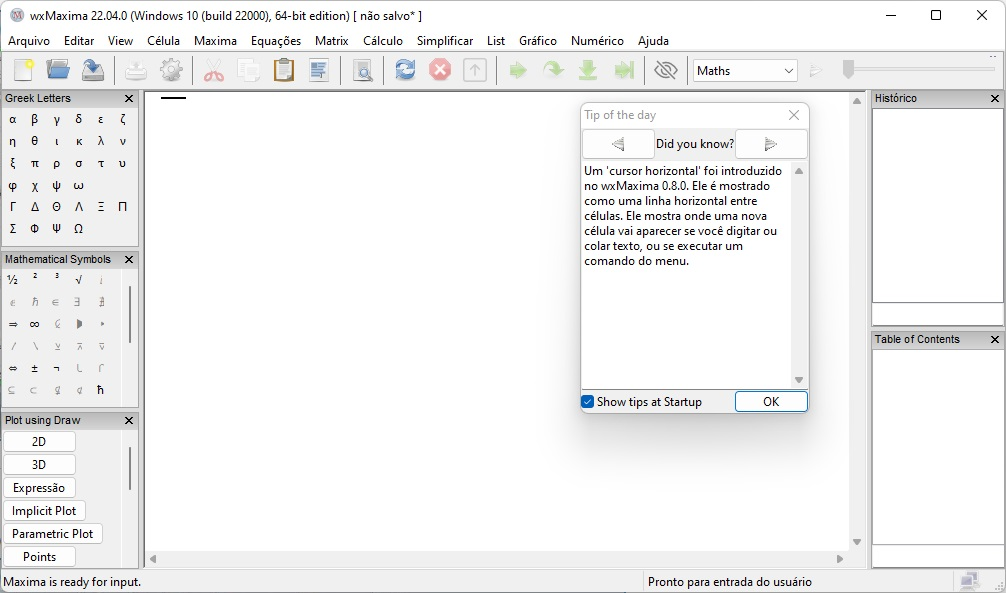
\includegraphics[scale=0.6]{tela-inicial.jpg}
	%\end{Center}
\end{figure}

\noindent A figura \ref{fig:selecao-tipos} mostra o recurso para escolher a opção de tipo de entrada no prompt, que podem ser
\begin{multicols}{2}
\begin{itemize}
\item tipo Texto
\item tipo Math
\item tipo Título
\item tipo Seção
\item tipo Subseção
\item tipo Subsubseção
\item head 5
\item head 6
\end{itemize}
\begin{figure}[H]
    %\centering
    \caption{Pré-seleção de tipo de entrada a ser inserida no prompt.}
        \label{fig:selecao-tipos}
    \begin{Center}
    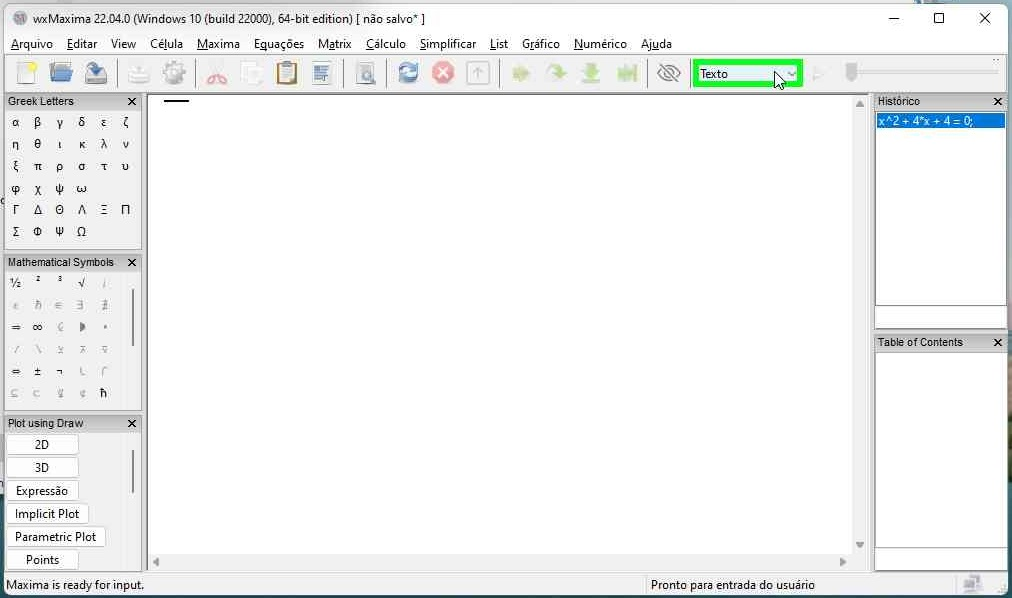
\includegraphics[scale=0.3]{selecao-tipos.jpg}
		\end{Center}
\end{figure}
\end{multicols}
%

\pagebreak
\noindent A figura \ref{fig:selecao-texto} mostra como escolher as opções de tipo de entrada no prompt para o caso de texto. Já a figura \ref{fig:selecao-math} mostra como escolher as opções de tipo de entrada no prompt para o caso de expressão algébrica.
	\begin{figure}[ht!]
    \centering
    \caption{Pré-seleção para inserir texto no prompt.}
        \label{fig:selecao-texto}
    %\begin{Center}
    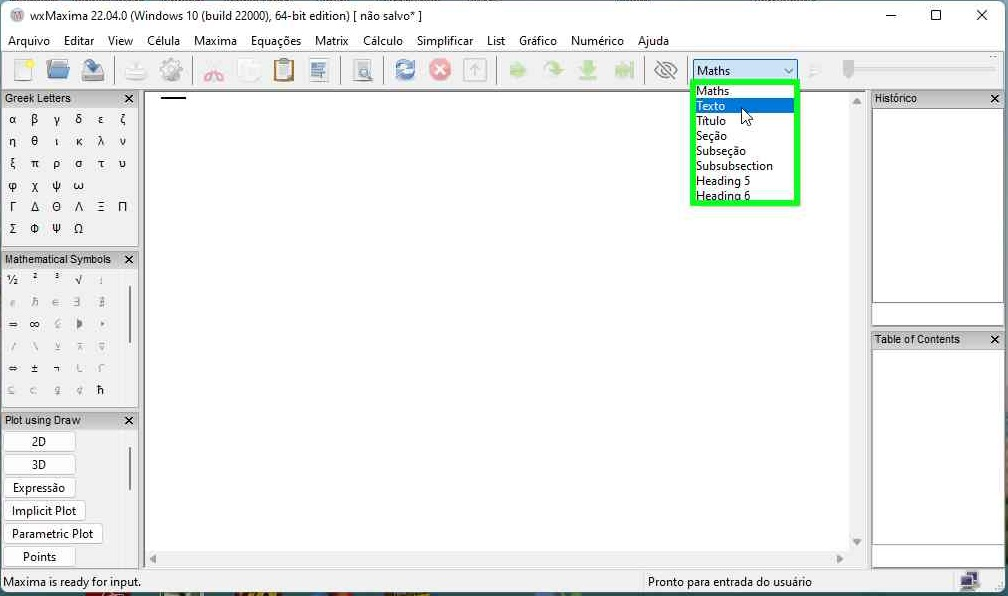
\includegraphics[scale=0.6]{selecao-texto.jpg}
	%\end{Center}
\end{figure}

\begin{figure}[H]
    \centering
    \caption{Pré-seleção para inserir expressão algébrica no prompt.}
        \label{fig:selecao-math}
    %\begin{Center}
    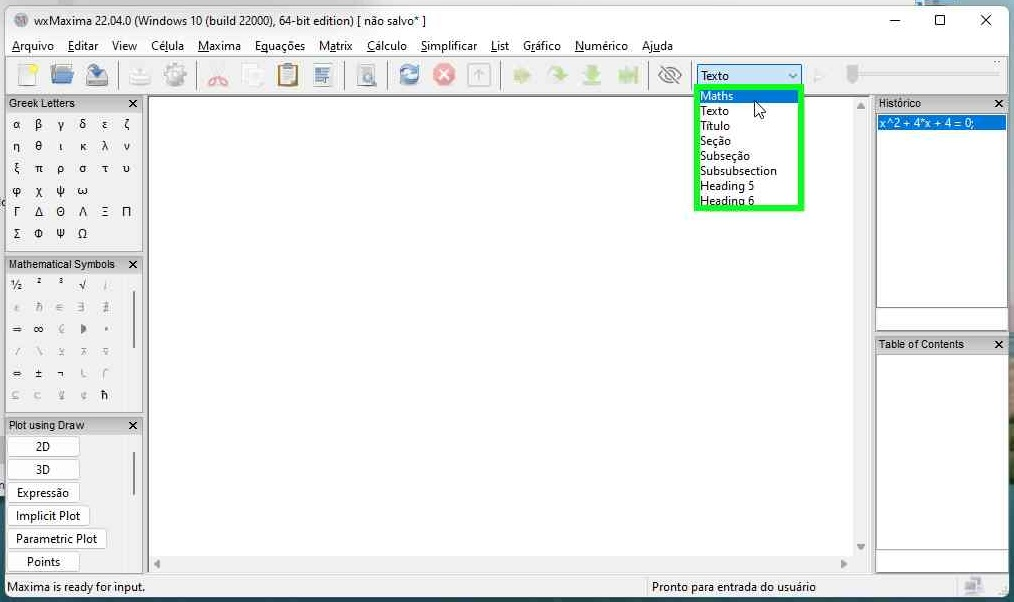
\includegraphics[scale=0.6]{selecao-math.jpg}
	%\end{Center}
\end{figure}
\pagebreak
Até agora nos ativemos a apresentar generalidades que subsidiarão o leitor durante sua jornada no aprendizado ou mesmo na utilização das técnicas de simulação aqui apresentadas no Maxima. Assunto que será objeto dos próximos capítulos.
%%%%%%%%%%
%%%%%%%%%%%%%%%%%%%%%%%%%%%%%%
\section{Um Pouco Sobre Ondas}
Há várias situações no dia a dia nas quais as coisas acontecem repentinamente, ou inesperadamente, vindo, depois a cessar seus efeitos, ou, em outros casos, repercutem mais além. É comum nos referirmos a isso com a expressão: "isso é apenas uma onda, logo passará". Isso, claro, devido a que tais situações são transitórias, exemplos: pandemias, endemias, o preço de commodities, tsunamis, terremotos, até notícias ou eventos cotidianos. Algumas vezes tais situações apresentam comportamento oscilante, como na superfície de um líquido em uma piscina, ou mesmo em fontes naturais de água, como em rios, mares e oceanos durante a passagem de uma embarcação.

É importante notar que existem características diferentes em tais situações. Alguns simplesmente oscilam ou vibram e em outros casos, além de oscilar ou vibrar, essa condição é posteriormente transmitida para outros locais do ambiente onde tais situações ocorrem. Neste segundo caso, diz-se que há uma propagação do fenômeno. De tal forma que, oscilação, onda, propagação são termos correlacionados.

Etimologicamente, a palavra onda teria a ver com o significado de algo que flutua na água. As descobertas e desenvolvimentos neste tema em seus primórdios derivaram do estudo dos sons musicais. Diz-se que o estudo moderno de ondas e acústica se originou com \emph{Galileu Galilei}.
A figura \ref{fig:mapa.ondas} apresenta a evolução, numa perspectiva histórica, do conhecimento científico desta temática, através da contribuição de vários investigadores.

\begin{figure}[htbp!]
	\centering
	\caption{Representação da evolução do conhecimento sobre ondas.}
	\label{fig:mapa.ondas}
	%\begin{Center}
	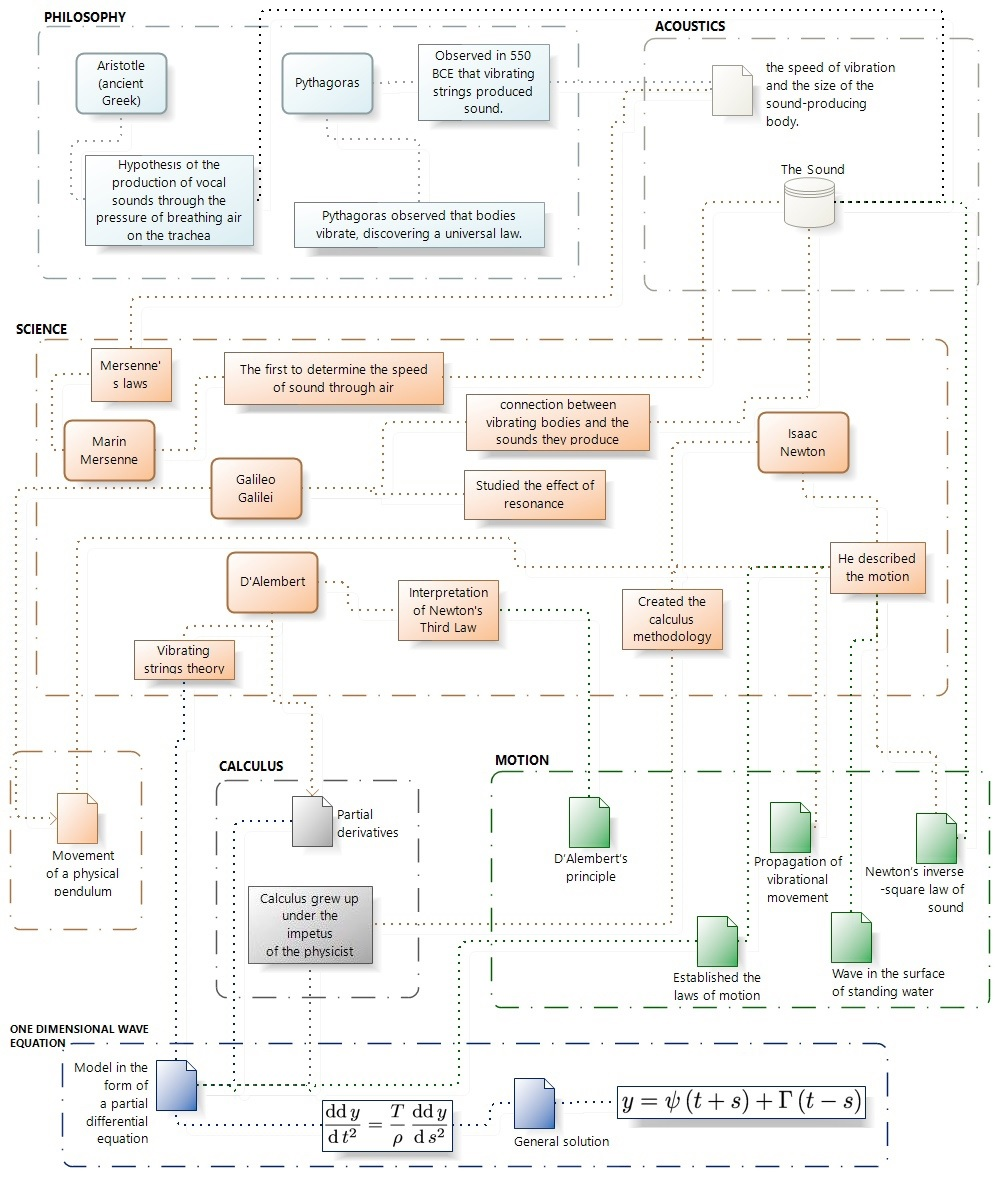
\includegraphics[width=0.95\textwidth,height=0.95\textheight]{sounds.jpg}
	%\end{Center}
\end{figure}
\newpage
%%%%%%%%
%%%%%%%%%%%%%%%%%%%%%%%%%%%%%%%%%%%%
\chapter{TRABALHANDO COM O wxMAXIMA}
A base de conhecimento do Maxima, de acordo com sua documentação, é organizada por meio de um conjunto de categorias, por exemplo: Expressões, Operadores, Avaliação de Expressões, Simplificação, Plotagem, etc.

Alguns elementos da estrutura do Maxima são estratégicos, como os \emph{flags}. Os \emph{flags} são os valores que determinadas variáveis internas do Maxima assumem de forma padrão ou conforme a definição do usuário. Exemplos:
\begin{itemize}
	\item {\texttt{showtime}} Tem valor \emph{false} como padrão. Quando definida para o valor \emph{true}, o tempo de processamento é impresso conjuntamente com cada saída de resultado.
	\begin{figure}[ht]
		\centering
		\caption{Efeito obtido após aplicar 'Showtime: true'}
		\label{fig:showtime-fig}
		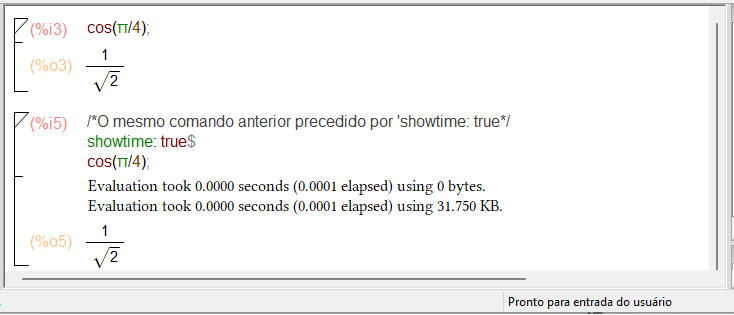
\includegraphics[width=0.7\linewidth]{showtime-fig}
	\end{figure}
	\item {\texttt{display2d}} Tem valor \emph{true} como padrão. Quando definido como  \emph{true} isso faz com que o Maxima apresente as expressões matemáticas na sua forma como as vemos nos livros.
	\begin{figure}[H]
		\centering
		\caption[Uso do variável "Display2D" com "flag" \emph{false}]{}
		\label{fig:display-2d}
		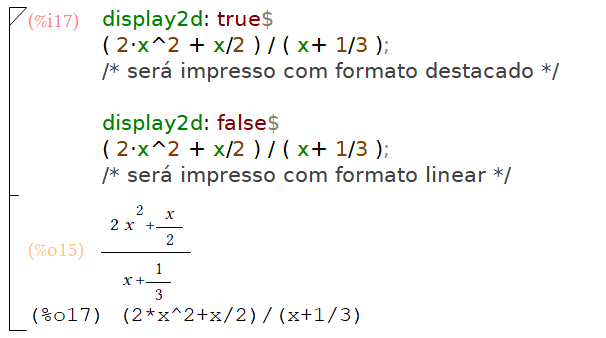
\includegraphics[width=0.7\linewidth]{display-2d}
	\end{figure}
	\item{\texttt{powerdisp}} description
\end{itemize}
Vamos tomar como primeiro exemplo a fórmula do teorema de Pitágoras. Vamos escrever no \emph{prompt} do wxMaxima a seguinte expressão: \textsf{c\^\ 2+b\^\ 2=a\^\ 2}
\begin{figure}[H]
    \centering
    \caption{Entrando uma expressão algébrica.}
        \label{fig:pitagoras}
    %\begin{Center}
    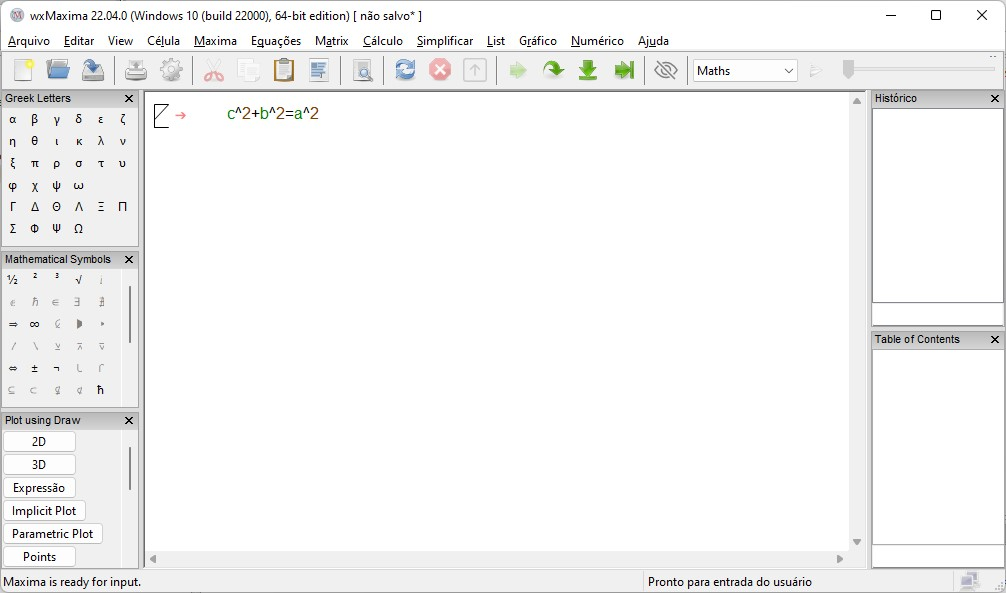
\includegraphics[scale=0.5]{pitagoras.jpg}
	%\end{Center}
\end{figure}

\noindent Essa expressão é o input do processo. O Maxima processará essa entrada após acionada a combinação de tecla \texttt{Shift+Enter} do que, em seguida, apresentará uma saída na área do \emph{prompt}, figura \ref{fig:pitagoras-2}.

\begin{figure}[ht]
    \centering
    \caption{Saída apresentada após após processamento da expressão algébrica entrada.}
        \label{fig:pitagoras-2}
    %\begin{Center}
    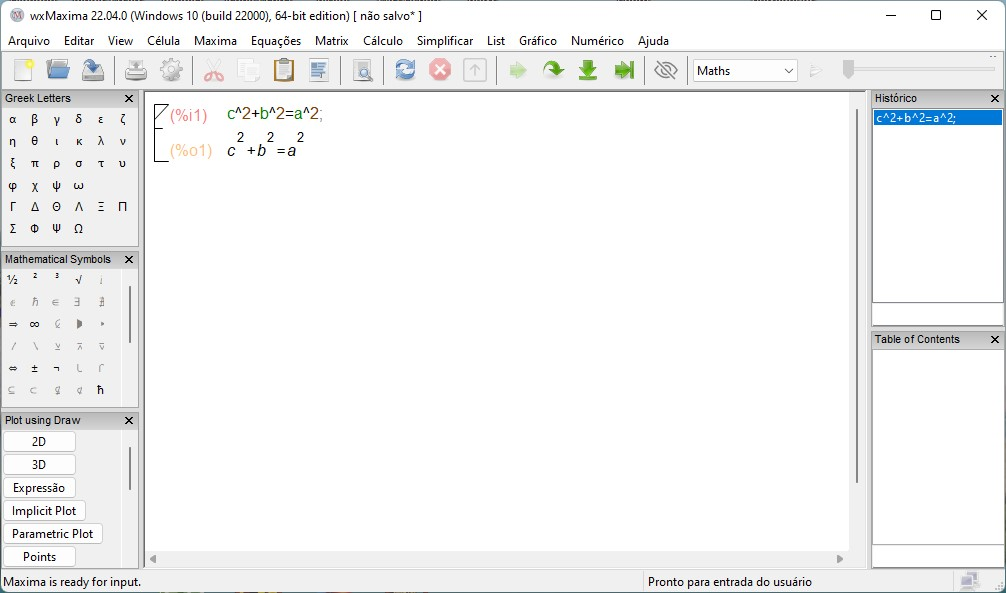
\includegraphics[scale=0.5]{pitagoras-2.jpg}
	%\end{Center}
\end{figure}
\pagebreak
\noindent Observe que a resposta disponibilizada recebe identificadores, tais que:

\begin{minipage}[]{4.000000em}\color{red}\bfseries (\% i1)	
\end{minipage}, indica que a expressão na linha é o \emph{input}, e 

%%%%

\begin{minipage}[]{4.000000em}\color{green}\bfseries (\% o1)	
\end{minipage}, indica que a expressao na linha é a saída (\emph{output}).


No Maxima é possível \emph{nomear uma expressão} de forma que possa ser reutilizada. Por exemplo, escrevendo no prompt a seguinte expressão: \textsf{pitg:c\^\ 2+b\^\ 2=a\^\ 2}. Observe o resultado disso na figura \ref{fig:pitagoras-3}.
\begin{figure}[ht]
    \centering
    \caption{Nomeando expressões.}
        \label{fig:pitagoras-3}
    %\begin{Center}
    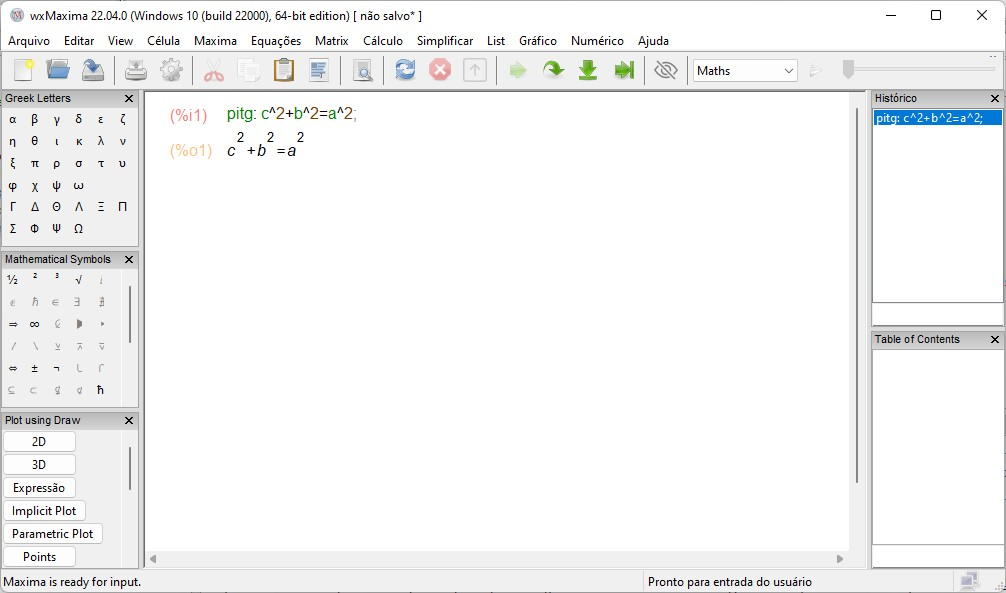
\includegraphics[scale=0.5]{pitagoras-3.jpg}
	%\end{Center}
\end{figure}


\noindent Essa ação de nomear as expressões algébricas é importante pois facilita a reutilização recorrente da fórmula. Por exemplo, com a seguinte expressão nomeada \textsf{sol1:solve(pitg,a)}. O termo \emph{solve} corresponde a uma fórmula (função) interna do Maxima. Os resultados aparecem na figura \ref{fig:pitagoras-4}. 
\begin{figure}[ht!]
    \centering
    \caption{Usando expressões.}
        \label{fig:pitagoras-4}
    %\begin{Center}
    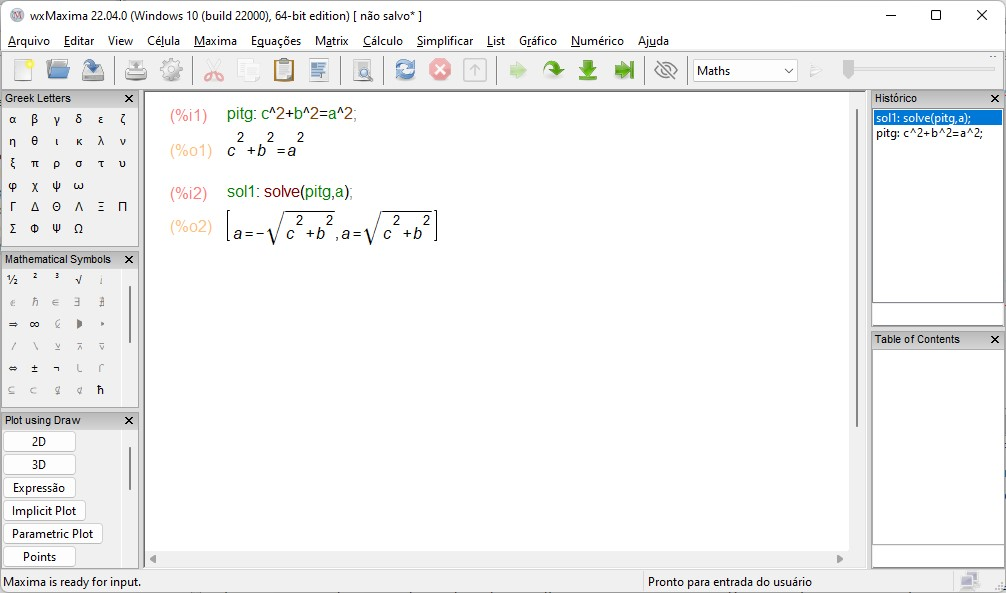
\includegraphics[scale=0.5]{pitagoras-4.jpg}
	%\end{Center}
\end{figure}
%%%

\pagebreak
\noindent Ao aplicar um termo \emph{solve}, o Maxima soluciona a expressão, no caso, \emph{pitg} para a literal \emph{a} tratando-a como a variável incógnita. Observe que o Maxiama retorna dois valores como saída, que era o que seria obtido, caso fossemos desenvolver a solução manualmente, e tais valores são apresentados no formato de uma lista ou vetor linha de dois elementos. 

Uma funcionalidade do Maxima é a possibilidade de recuperar um elemento de um vetor ou lista. Por exemplo, vamos recuperar uma das soluções obtidas do passo anterior. Vamos usar a seguinte sintaxe como \emph{input}: \textsf{sol2:sol1[2];}. O resultado é mostrado na figura \ref{fig:pitagoras-5}
\begin{figure}[ht!]
    \centering
    \caption{Obtendo o valor de um elemento de uma lista.}
        \label{fig:pitagoras-5}
    %\begin{Center}
    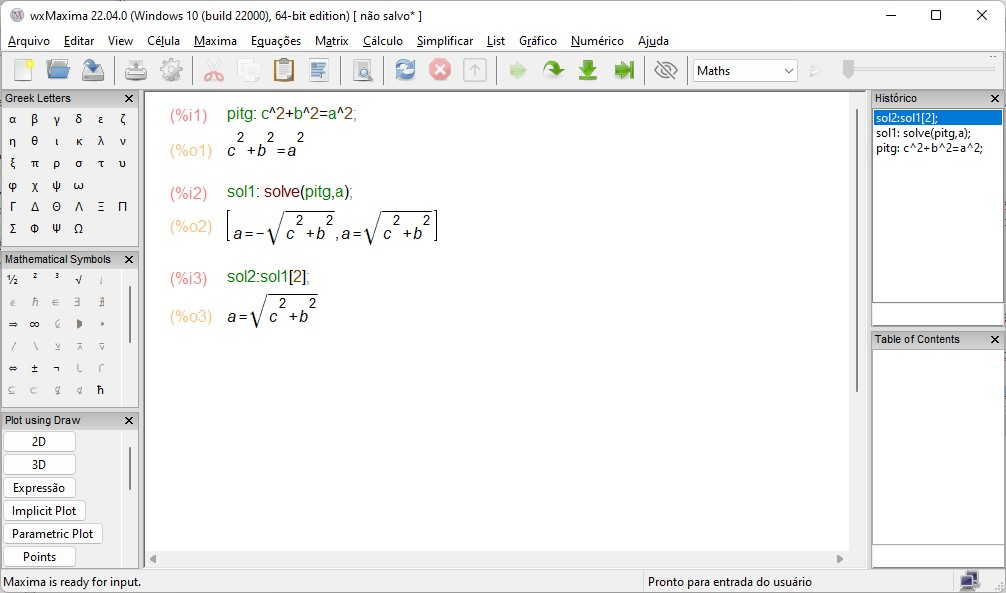
\includegraphics[scale=0.5]{pitagoras-5.jpg}
	%\end{Center}
\end{figure}
%%%

\noindent Observe que o Maxima atribuiu à expressão \textsf{sol2} o valor do segundo elemento do vetor \textsf{sol1}, ou seja, o valor do elemento de índice \textsf{[2]}

O Maxima também suporta um ambiente de texto, misturado entre os comandos algébricos, recurso muito útil no caso de o usuário precisar de documentar seu trabalho com texto explicativo e formatado. Por exemplo vamos colocar um título introdutório em nossa tela e uma texto explicativo intermediário. 

\noindent O título será um texto a ser inserido antes da primeira célula. Uma célula é o espaço delimitado pelo seletor lateral (parentese "exótico" que aparece à esquerda das expressões) idêntico ao desenho abaizo
\begin{figure}[h]
	\centering
		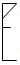
\includegraphics[scale=0.6]{seletor.jpg}
	\label{fig:seletor}
\end{figure}

\noindent O cursor horizontal deve ser transportado com auxílio das teclas de navegação do teclado, ou diretamente com o uso de dispositivo apontador ("mouse"), ver figura \ref{fig:curso-hrizontal-2}. 

\begin{figure*}[hp]
	\centering
	\caption{Posição sugerida para escrever um título}
		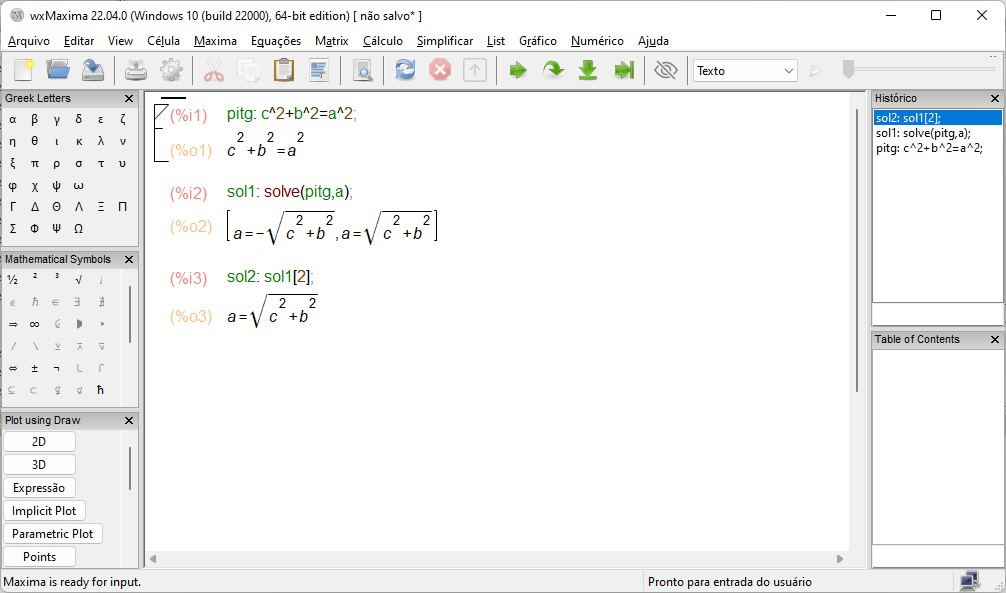
\includegraphics[width=0.80\textwidth]{curso-hrizontal-2.jpg}
	\label{fig:curso-hrizontal-2}
\end{figure*}

Em seguida digita-se o texto pretendido para título:
\begin{figure}[ht!]
	\centering
		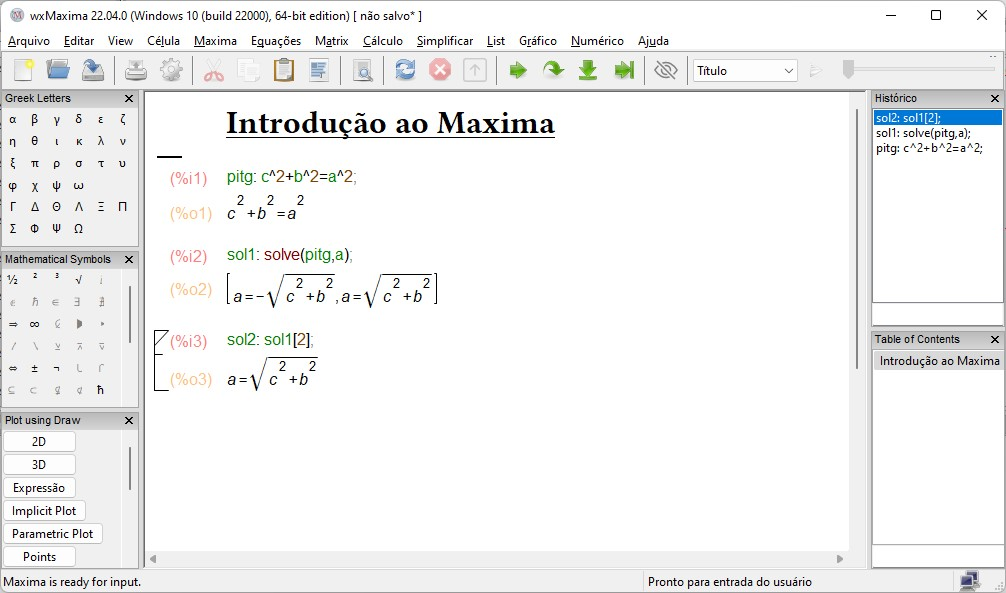
\includegraphics[width=0.80\textwidth]{introducao-maxima.jpg}
	\caption{Resultado da inserção de título}
	\label{fig:introducao-maxima}
\end{figure}
\clearpage

E, digita-se um texto explicativo pretendido:
\begin{figure}[ht!]
	\centering
	\caption{Resultado da inserção de texto comum}
		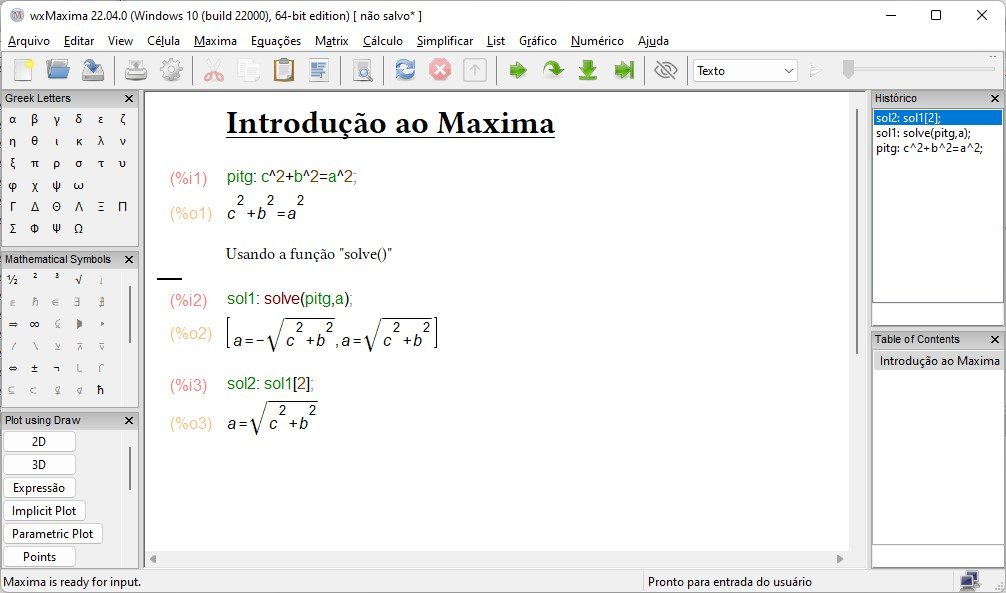
\includegraphics[width=0.80\textwidth]{usando-solve.jpg}
	\label{fig:usando-solve}
\end{figure}
\clearpage
%\pagebreak
Por hora esses são os conhecimentos sobre o Maxima, indispensáveis para imergir sobre o universo de possibilidades. São conhecimentos básicos e no decorrer dos outros capítulos estaremos apresentando outos recursos básicos ou mais complexos, conforme a exigência do contexto.
\chapter{ESTUDO DAS FUNÇÕES TRIGONOMÉTRICAS}
\label{estudos}
\newcounter{exemplos}
\setcounter{exemplos}{1}
\newcounter{exercicios}
\setcounter{exercicios}{1}
As funções trigonométricas tiveram suas origens no estudo das medidas astronômicas, e elas são de suma importância para as ciências em geral, dado que as suas características permitem de serem utilizadas para representar o comportamento de diversos sistemas reais. 

Elas são desenvolvidas por meio do estudo da circunferência de raio unitário com relação às dimensões em um determinado sistema de cordas. A palavra \emph{seno} etimologicamente significa meia corda. As funções trigonométricas também tem relações  com a geometria por meio das razões trigonométricas no triângulo retângulo.

	As funções trigonométricas são ditas \emph{periódicas}. Uma função \(f:\mathds{R} \rightarrow \mathds{R}\) é dita periódica com período \(T > 0\)  se:
\begin{enumerate}{ }{ }
	\item  seu domínio contém \(x+T\) sempre que contém \(x\), e se
	\item \(f(x)=f(x+T)\) para todo \(x\) pertencente ao domínio de \(f\).
\end{enumerate}

\section{As Funções Trigonométricas no Maxima}
No Maxima você irá se referir às funções trigonométricas usando as seguintes sintaxes.
\begin{itemize}
	\item seno: \textsf{f(x):=sin(x)};
	\item cosseno: \textsf{f(x):=cos(x)};
	\item tangente: \textsf{f(x):=tan(x)},
\end{itemize}
onde \emph{x}, ou seja, o argumento de função, deve ser entendido como medida de arco expressa em radianos. O Maxima usa ":=" para definir funções.

Vamos a uma ilustração. Vamos construir uma tabela dessas funções, para alguns pouco valores de arco.
\clearpage
\pagebreak{}
{ {\scshape Exemplo \thesection.\theexemplos: Construindo uma tabela}}\\
\noindent

%%%%%%%%
%% INPUT:
\noindent
/*Definição\ das\ funções\ trigonométricas\ no\ ambiente.\ */

\noindent
%%%%
\begin{minipage}[]{\textwidth}\color{blue}
%/*Definição\ das\ funções\ trigonométricas\ no\ ambiente.\ */\\
f(x):=sin(x)\$;\ g(x):=cos(x)\$
\end{minipage}
\noindent%
\\


\noindent
%%%%%%%%
%% INPUT:
/*Configuração\ do\ ambiente\ para\ calculos\ simbólicos\ (não\ numérico).\ */
\noindent%
\\


\noindent /*\-inicializa\ incremento\ para\ cálculo\ \ do\ domínio\ de\ valores\ para\ "x".\ */\\
\noindent
\begin{minipage}[]{\textwidth}\color{blue}
arc:\ensuremath{\pi}/12\ \$\ \ \ \ \ \ \ \ \ \ \ \ \ \ \ \\
\end{minipage}
%%%%
\noindent%
\\


\noindent /*-gera\ lista\ com\ os\ elementos\ para\ o\ cabeçalho\ de\ colunas.\ */\\
\begin{minipage}[]{\textwidth}\color{blue}
cabeçalhoDaTabela:\ ["Arco(rad)",\ arc,\ 2*arc,\ 3*arc,\ 4*arc\ ]\$\ \ 
\end{minipage}
\noindent%
\\


\noindent /*a\ partir\ daqui\ o\ cálculo\ será\ numérico.\ */\\
%%%%%%%%
%% INPUT:	
\noindent
\begin{minipage}[]{\textwidth}\color{blue}
numer:\ true\$\ \\
arc:\ensuremath{\pi}/12\ \$
\end{minipage}
\\
\noindent%


\noindent /*construindo\ lista\ de\ valores\ de\ seno.\ */\\
%%%%%%%%
%% INPUT:
\noindent
\begin{minipage}[]{\textwidth}\color{blue}
linha1:makelist(f(x),x,\ [arc,2*arc,3*arc,4*arc])\$\ \ \ \ \ \ \ \ \ \ \ \ \\
\end{minipage}
\\
\noindent%


\noindent /*a\ lista\ é\ reconstruída\ para\ incluir\ nela\ um\ cabeçalho\ de\ linha.\ */\\
\begin{minipage}[]{\textwidth}\color{blue}
linha1:["Seno",\ linha1[1],\ linha1[2],\ linha1[3],\ linha1[4]]\$\ \ \ \ \ 
\end{minipage}
\\
\noindent%


\noindent /*construindo\ lista\ de\ valores\ de\ cosseno.\ */\\
%%%%%%%%
%% INPUT:
\begin{minipage}[]{\textwidth}\color{blue}
linha2:makelist(g(x),x,\ [arc,2*arc,3*arc,4*arc])\$\ \ \ \ \ \ \ \ \ \ \\
\end{minipage}
\noindent%


\noindent/*a\ lista\ é\ reconstruída\ para\ incluir\ nela\ um\ cabeçalho\ de\ linha.\ */\\
\begin{minipage}[]{\textwidth}\color{blue}
linha2:["Cosseno",linha2[1],\ linha2[2],\ linha2[3],\ linha2[4]]\$\ \ 
\end{minipage}
\\
\noindent%


\noindent /*----\ Saída\ dos\ Resultados\ ---------------------------------*/\\
%%%%%%%%
%% INPUT:
\noindent%


\noindent /*definindo\ a\ precisão\ numérica.\ */\\
%%%%%%%%
%% INPUT:
\begin{minipage}[]{\textwidth}\color{blue}
fpprintprec\ :\ 3\$
\end{minipage}
\\
\noindent%


\noindent /*formato\ usando\ a\ função\ table\_form().\ \ */\\
%%%%%%%%
%% INPUT:
\begin{minipage}[]{\textwidth}\color{blue}
table\_form([cabeçalhoDaTabela,\ linha1,\ linha2]);
\end{minipage}
\\
\noindent%


\noindent /*formato\ usando\ a\ função\ matrix().\ \ */\\
%%%%%%%%
%% INPUT:
\begin{minipage}[]{\textwidth}\color{blue}
matrix(cabeçalhoDaTabela,\ linha1,\ linha2);
\end{minipage}
%%
% 
% $$e^{\pi i} + 1 = 0$$
% 
%%%%%%
\clearpage
Copie na memória do seu computador as linhas de comando desse exemplo \thesection.\theexemplos\, e cole-as na janela do wxMaxima, avalie com o comando de teclado \texttt{Shift+Enter} e veja o resultado, deverá ser idêntico ao da figura \ref{fig:exemplo331}. O conteúdo limitado entre '/* */' é interpretado apenas como texto de comentários.
\begin{figure}[H]
    \centering
    \caption{Resultado do exemplo na janela do wxMaxima.}
        \label{fig:exemplo331}
    %\begin{Center}
    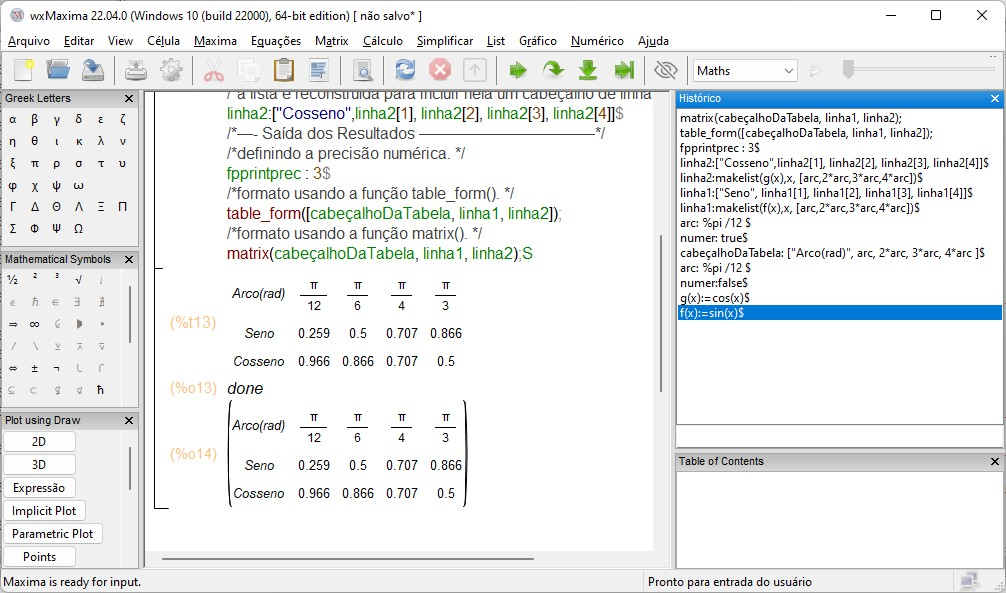
\includegraphics[scale=0.6]{exemplo331.jpg}
	%\end{Center}
\end{figure}
\vspace{20pt}
%%% pesquisar evfun no maxima  - distribute_over	- cabs - Trigonometric functions
%%%
\begin{tcolorbox}[enhanced jigsaw, colback=gray!30, colframe=Maroon,width=1\textwidth, arc=3mm, auto outer arc, boxrule=5pt, drop shadow={Maroon!50!gray!80}]
  	\noindent
	Exercício \thesection.\theexercicios: No encejo do exemplo \thesection.\theexemplos, acrescente ou modifique comandos de forma que apareçam,
	\begin{enumerate}
	\item uma linha correspondente aos valores de tangente e, 
	\item uma coluna correspondente ao arco igual a $\frac{5\,\pi}{12}$.
	\end{enumerate}
\end{tcolorbox}
%%%
\section{Manipulando Expressões Trigonométricas}
Esta seção será dedicada a mostrar como trabalhar expressões trigonométricas no Maxima. O Maxima é constituído de pacotes de comandos (\emph{packages})Há dois tipos de comandos específicos: as \emph{tags} (ou variáveis de controle) e as funções. 
Algumas funções possuem o mesmo nome das tags. Geralmente as tags servem para comutar dois estados ,o "true" ou "false", um desses será o valor padrão (\emph{default}).
%%%%
%%%% SOMA DE ARCOS
%%%%
\subsection{Soma de Arcos}
Usa-se a função: \texttt{trigexpand}.

\noindent
%%%%%%%%
%% INPUT:
\begin{minipage}[t]{4.000000em}\color{red}\bfseries (\% i2)	\end{minipage}
\begin{minipage}[t]{\textwidth}\color{blue} trigexpand(sin(a+b)); \end{minipage}
%%%% OUTPUT:
\begin{minipage}[]{4.000000em}\color{green}\bfseries (\% o2) \end{minipage}
\begin{minipage}[]{4.000000em}  $\mathrm{\displaystyle \cos{(a)} \sin{(b)}+\sin{(a)} \cos{(b)}\mbox{}} $\end{minipage}
%%%%%%%%%%%%%%%%

%%%%
%%%% ARCO METADE
%%%%
\subsection{Arco Metade}
Usa-se a função seno com o argumento arco metade, porém é preciso obedecer certar regras, como mostrado seguir.

%%%%%%%%
%% INPUT:
\noindent\begin{minipage}[hp]{4.000000em}\color{red}\bfseries (\% i4)	\end{minipage}
\noindent /*'halfangles',\ se\ 'true'\ o\ Maxima\ manipulará*/\\
/*o\ arco\ metade\ como\ expressão\ algébrica,\ senão\ o\ fará\ como\ texto.*/\\
\begin{minipage}[]{\textwidth}\color{blue}\hspace{4em} halfangles:\ true\$\mbox{}\\
\end{minipage}
\\
%%%
\noindent /*\ \%pi\ é\ o\ nome\ da\ contante\ matemática\ no\ ambiente\ do\ Maxima.*/\\
/*Se\ '\%piargs'\ for\ definido\ para\ 'true'\ ,\ então\ será\ manipulado\ como\ valor*/\\
\begin{minipage}[]{\textwidth}\color{blue}
\hspace{4em}\%piargs:\ true\$\\
\end{minipage}
\\
\noindent /*'assume'\ é\ uma\ função\ interna\ cuja\ finalidade\ é\ de*/\\
/*estabelecer\ um\ domínio\ de\ valores\ para\ um\ contexto*/\\
\begin{minipage}[]{\textwidth}\color{blue}
\hspace{4em} assume(a\ensuremath{>}0,\ a\ensuremath{<}2*\%pi)\$\\
\end{minipage}
\\
\noindent /*Seno\ do\ arco\ metade*/\\
\begin{minipage}[]{\textwidth}\color{blue}
\hspace{4em} sin(a/2);\\
\end{minipage}
%%%% OUTPUT:
\begin{minipage}[]{4.000000em}\color{green}\bfseries (\% o4) \end{minipage}
\begin{minipage}[]{4.000000em}  $\mathrm{\displaystyle \frac{\sqrt{1-\cos{(a)}}}{\sqrt{2}}\mbox{}} $\end{minipage}
%%%%%%%%%%%%%%%%
%%%%
%%%% ARCO DUPLO
%%%%
\subsection{Arco Duplo}

\noindent\begin{minipage}[hp]{4.000000em}\color{red}\bfseries (\% i13)	\end{minipage}
\noindent /*Se\ "trigexpand"\ estiver\ comutado\ (definido)\ para\ "true"\ */\\
/*então,\ se\ "trigexpandtimes"\ estiver\ definido\ para\ "true"\ então\ */\\
/*o\ Maxima\ irá\ expandir\ a\ expressão\ do\ arco\ duplo.*/\\
%%%%%%%%
%% INPUT:
\begin{minipage}[]{\textwidth}\color{blue}
\hspace{4em} trigexpand:\ true\$

\hspace{4em} trigexpandtimes:\ true\$
\end{minipage}
\\


\noindent /*Seno\ do\ arco\ duplo.*/\\
\begin{minipage}[]{\textwidth}\color{blue}
\hspace{4em} sin(2*\ensuremath{\alpha});\\
\end{minipage}
%%%% OUTPUT:
\begin{minipage}[]{4.000000em}\color{green}\bfseries (\% o13) \end{minipage}
\begin{minipage}[]{\textwidth}\color{blue}
$\displaystyle 2 \cos{\left( \alpha \right) } \sin{\left( \alpha \right) }\mbox{}
$
\end{minipage}
%%%%%%%%%%%%%%%%
%%%%
%%%% CONSTRUÇÃO DE GRÁFICOS
%%%%
\section{Construção de Gráficos}

\chapter{DESCRIÇÕES DE MOVIMENTOS ONDULATÓRIOS}
\section{Abordagem Matemática}
A concepção matemática mais simples de uma onda é o traçado, no plano cartesiano, das funções seno ou cosseno. Assim, vamos tomar como modelo ou perfil a expressão da função senoidal ou, harmônica como também é chamada para descrever o movimento ondulatório. 

Considerando-se a variável independente \(\theta\), em radianos, coincidindo com o eixo das abcissas do plano cartesiano, então teríamos a expressão da função seno na forma
\begin{equation*}
	\xi \qty(\theta) =\xi_0 \sin\theta \text{,}
\end{equation*}
\begin{multicols}{2}
\noindent onde,
	\begin{enumerate}
		\item \( \xi\qty(\theta) \) é o valor da função, corresponde a ordenada ou cota no gráfico da figura \ref{fig:geogebra-seno}. Poderia estar representando a \emph{amplitude} local de uma propriedade física, e
		\item  o arco, \( \theta \), do qual está sendo calculado o seno, é \emph{a fase}. É um valor de arco cuja amplitude associada será sempre de mesmo valor à medida que se evolua a função \( \xi \)  por meio de ciclos iguais a \( 2\,\pi\, \mathrm{rad} \).
	\end{enumerate}

	\begin{figure}[H]
		\centering
		\caption[]{Perfil da função harmônica.}
		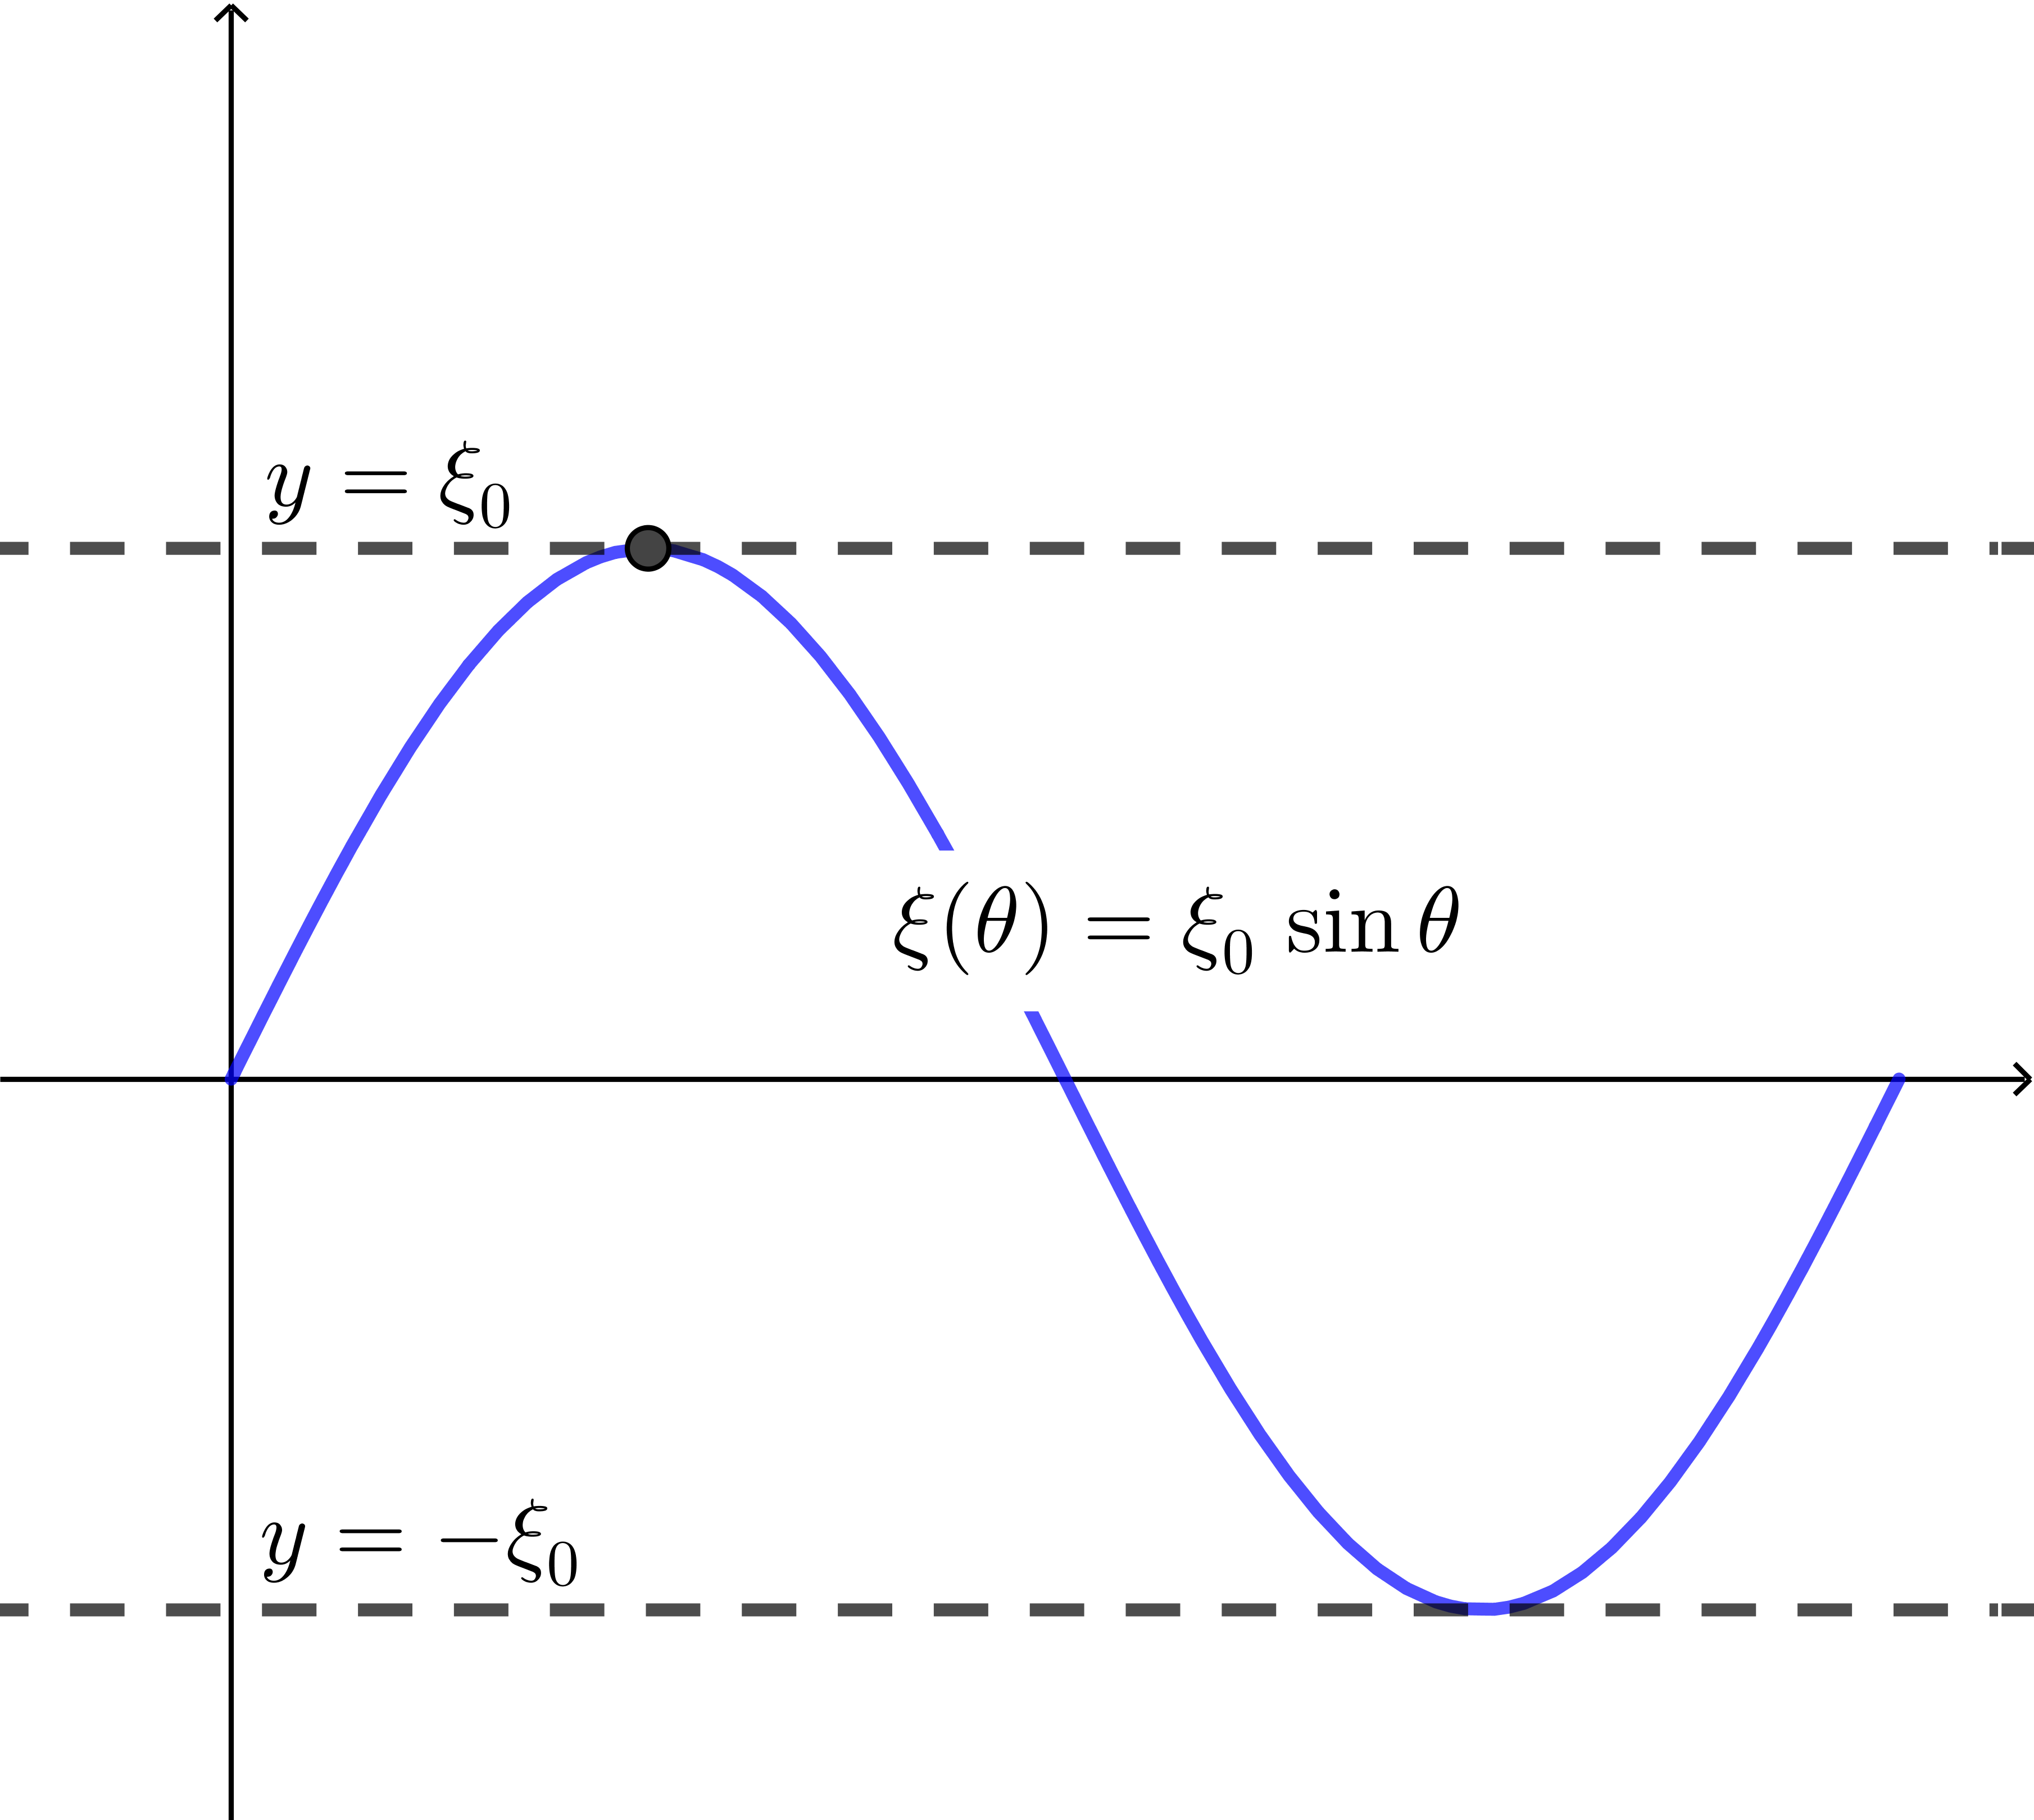
\includegraphics[scale=.07]{geogebra-seno}
		\label{fig:geogebra-seno}
	\end{figure}
	
	
\end{multicols}
\noindent Um gráfico dessa função está representado na figura \ref{fig:geogebra-seno}.

Vamos supor que tenhamos agora uma outra função na forma
\begin{equation*}
	\xi_1 \qty(\theta) =\xi_0 \sin\qty(\theta- \delta)\text{.}
\end{equation*} Ela seria representada na forma do gráfico da figura \ref{fig:geogebra-seno-2}, ou seja, uma senoide deslocada da origem dos eixos à direita.
\begin{figure}[H]
	\centering
	\caption[]{Gráfico de um perfil de uma função harmônica deslocado da origem do eixo das abcissas.}
	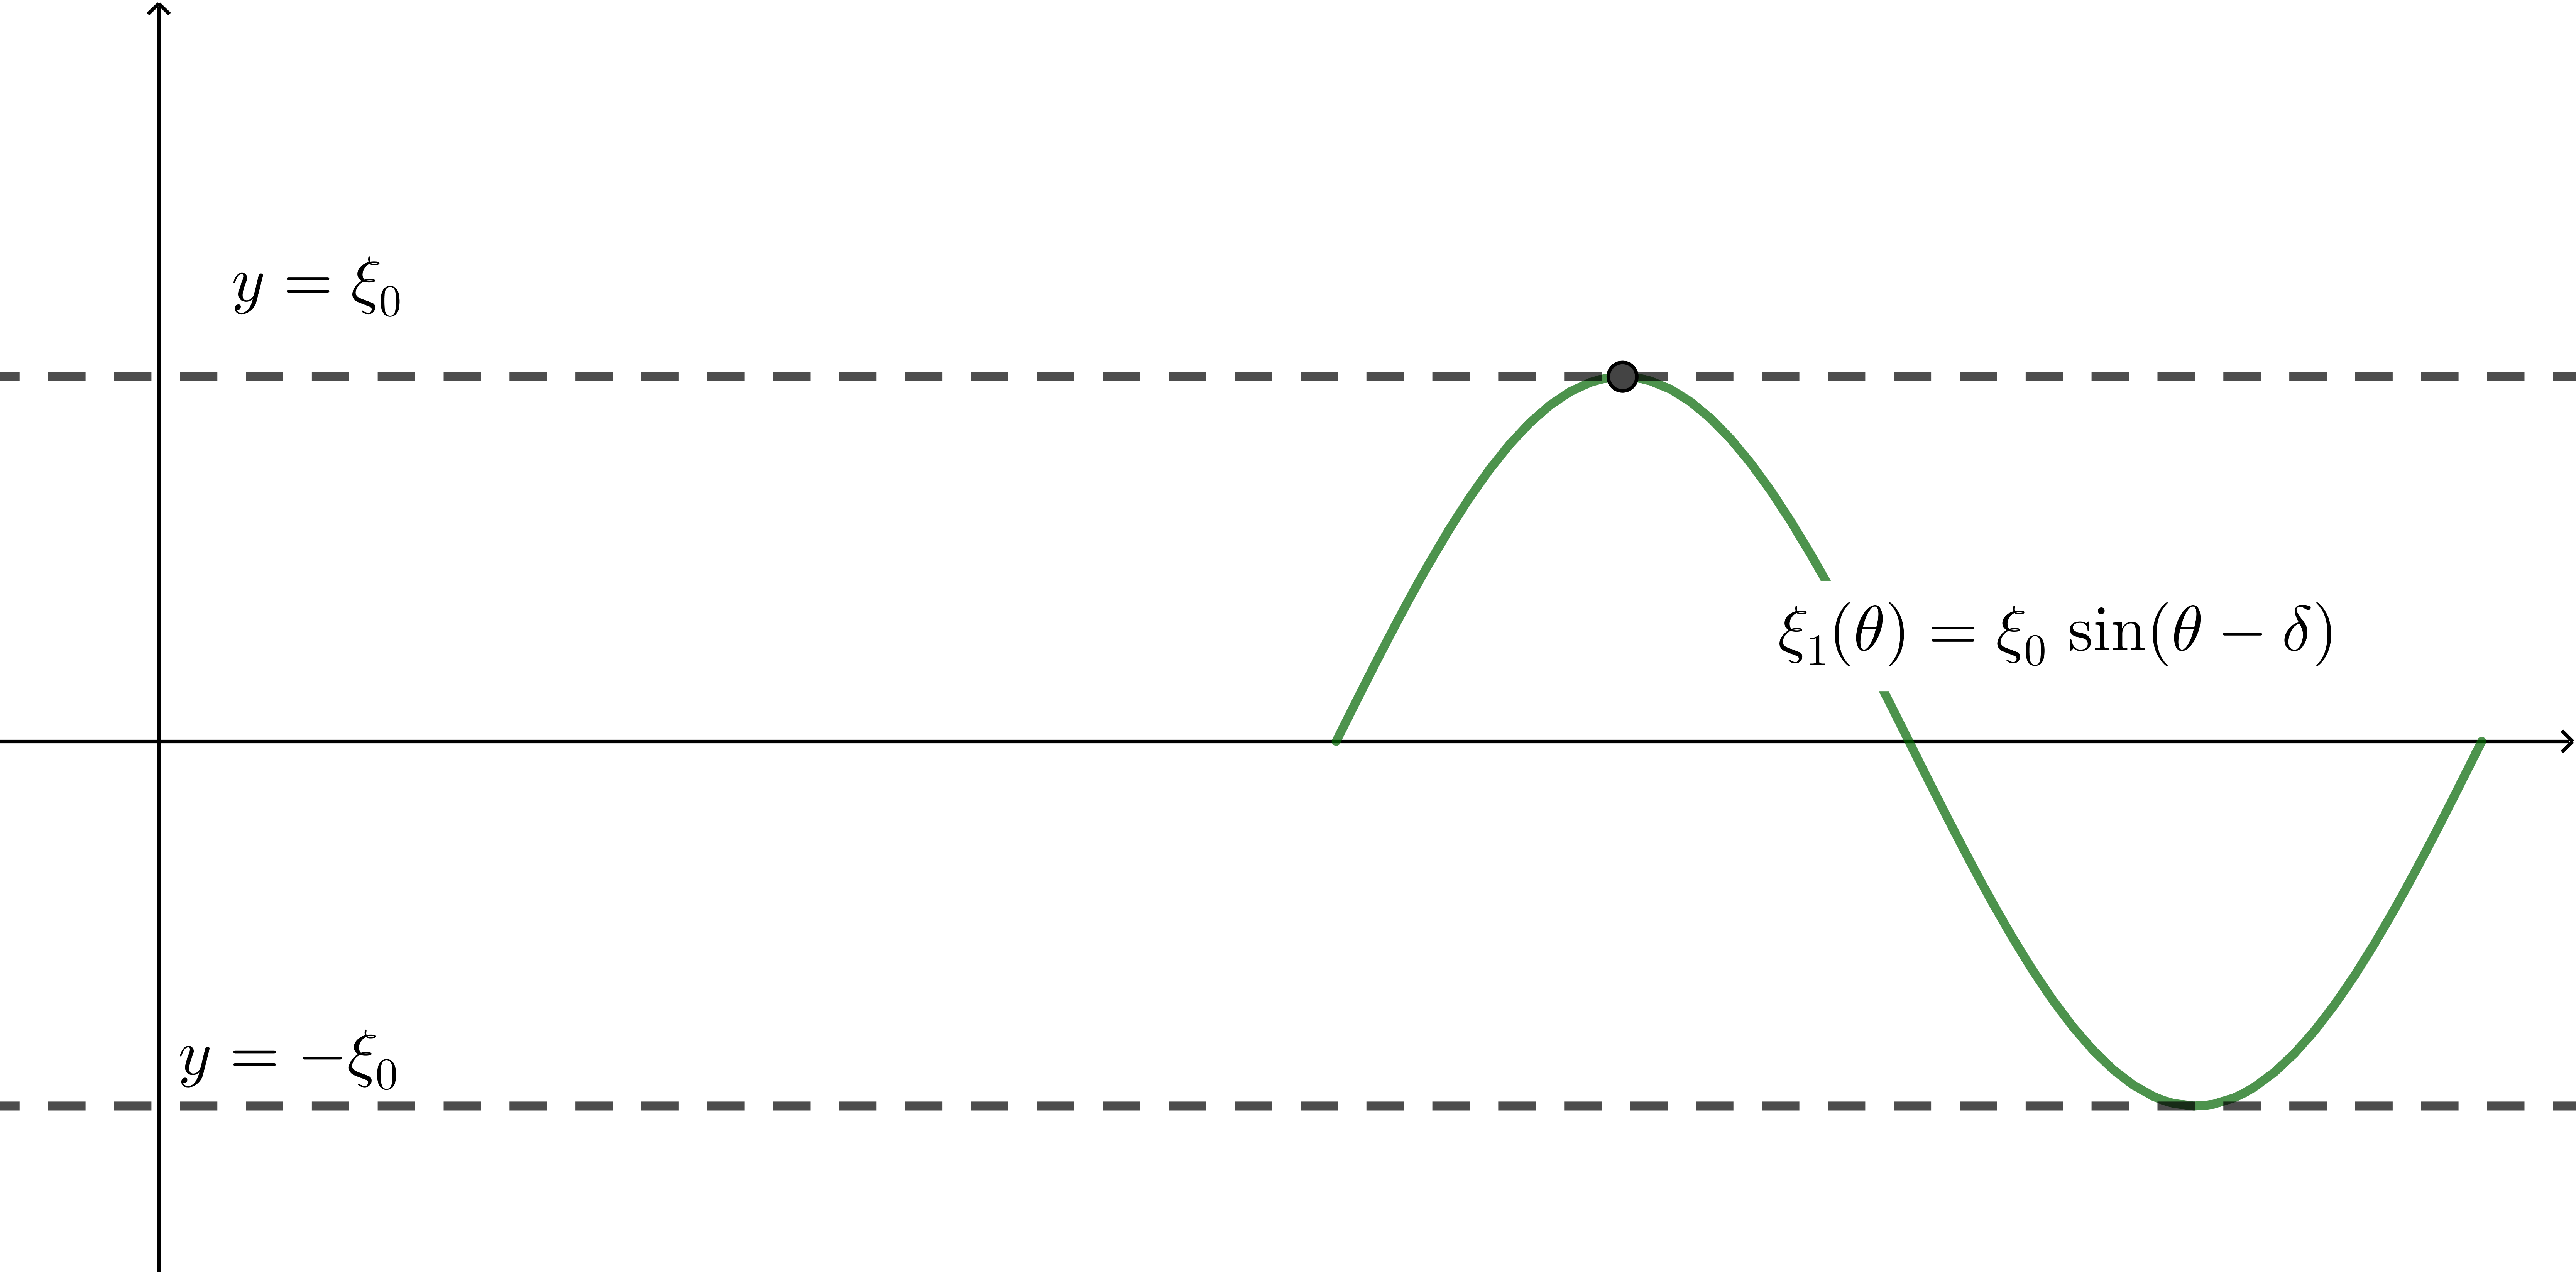
\includegraphics[width=0.7\linewidth]{geogebra-seno-2}
	\label{fig:geogebra-seno-2}
\end{figure}
Os dois gráficos anteriores, apresentados juntos como mostrado na figura \ref{fig:geogebra-seno-3}, permite-nos vislumbrar que ambos são semelhantes na forma, estão deslocados no espaço (eixo \( \theta \)) de uma distância igual a \( \delta \).
\begin{figure}[ht]
	\centering
		\caption[]{Confrontação dos gráficos de duas funções harmônica inter deslocadas.}
	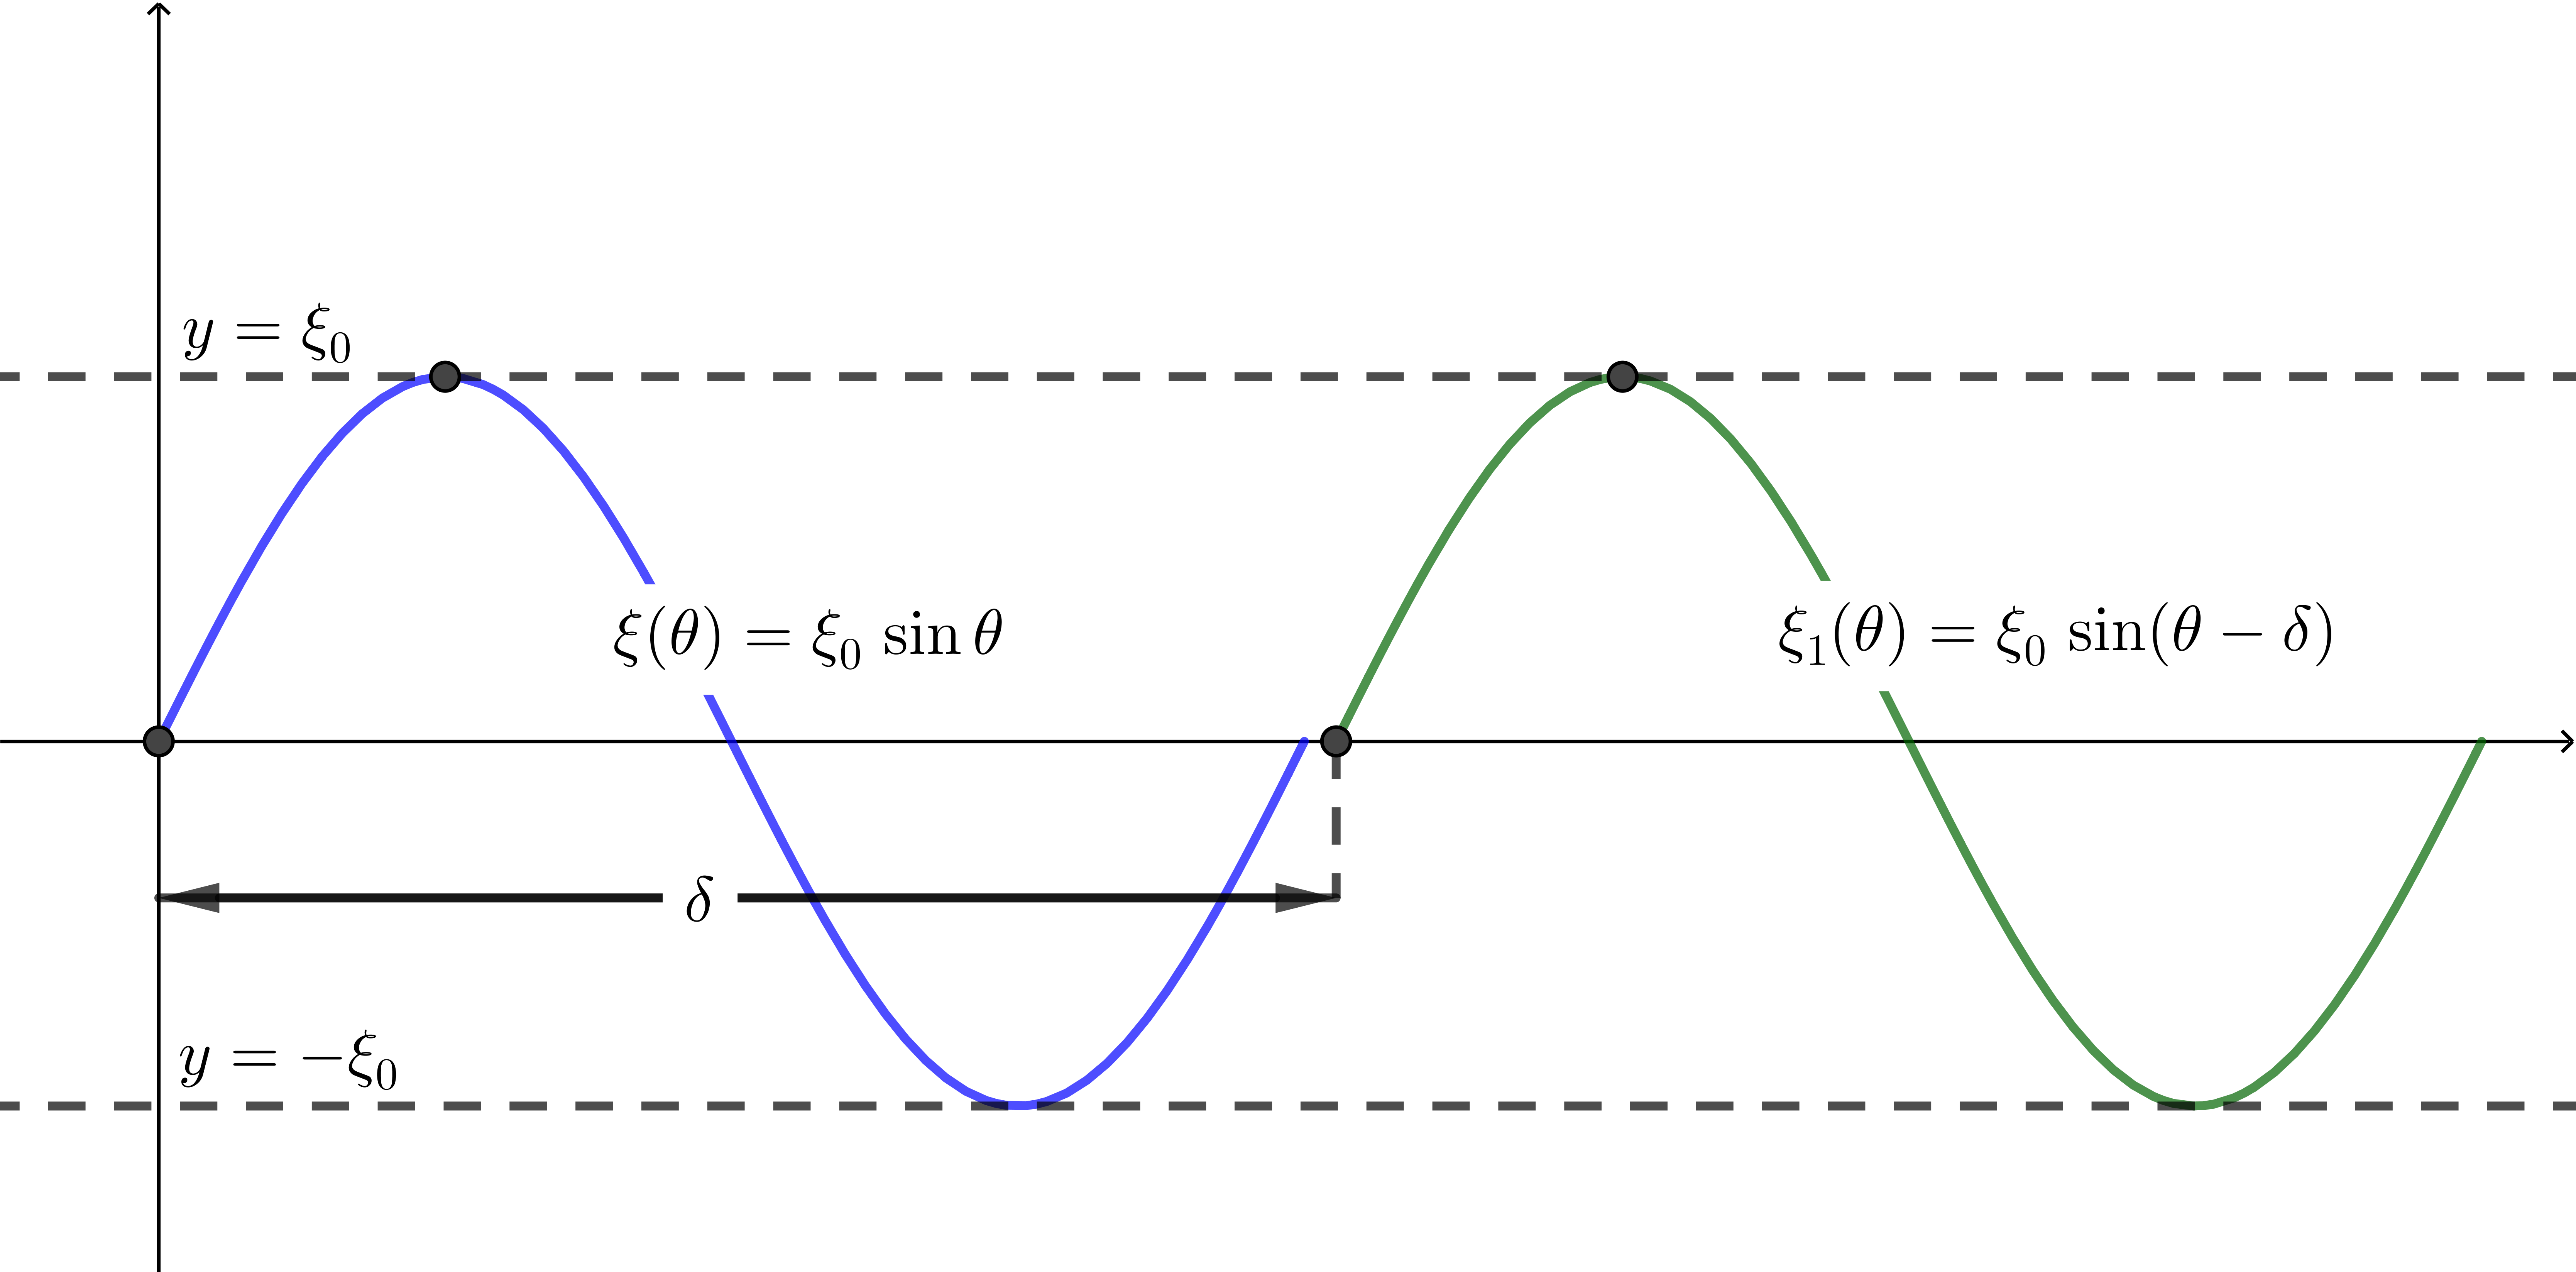
\includegraphics[width=0.7\linewidth]{geogebra-seno-3}
	\label{fig:geogebra-seno-3}
\end{figure}
Ou seja, diz-se que a função \( \xi_1 \) é uma translação de \( \xi \)

Estamos tratando uma variável independente que representa medidas em radianos, que é a variável  \( \theta \). Então temos que passar a adotar um medida de distância para melhor representar os sistemas físicos daqui em diante.

Podemos fazer a transformação matemática \( \theta = k\, x - \delta\), onde a variável \( x \) estará com aí presente para representar de fato uma posição, agora no eixo X.  

Fisicamente falando, o traçado da senoide como representando o efeito de uma onda tem origem na posição onde uma fonte impõe oscilação ou vibração ao meio. A partir daí o meio absorve e ao mesmo tempo transmite a energia e quantidade de movimento para sua vizinhança também na forma de oscilação local.

A presença de um fenômeno físico ondulatório cujo perfil da onda estaria sendo esboçado pela senoide do lado direito da figura \ref{fig:geogebra-seno-3}, sugere que ele, o perfil, é uma repetição do que está à esquerda, ou seja o perfil atual é uma repetição gráfica e manterá a sua extensão horizontal em radianos, durante as repetições sucessivas. Então, para um determinado valor de \( x \) é verdadeiro escrevermos a igualdade \( \sin\qty(2\,\pi + k\,x - \delta) = \sin\qty(k\,x-\delta)\), qualquer que seja o valor de \( x \).

Na forma algébrica, temos:
\[ \xi \qty(x) = \xi_0 \sin \qty( k\, x - \delta)\]
ou 
\begin{equation}\label{eq-delta/k}
	\xi \qty(x) =  \xi_0 \sin k \qty(x- \frac{\delta}{k})\text{,}
\end{equation}
e da mesma forma
\[ \xi\qty(x)=\xi_0\sin k\qty(\frac{2\,\pi}{k}+ x- \frac{\delta}{k})\text{,} \]
%%%%%%%%%%%%%%%%%%%%%%%%%%%%
Se considerarmos neste momento, o \( k \) como um coeficiente contante, então a quantidade \(\frac{2\,\pi}{k}  \) também o será. Tal quantidade, a qual é da mesma grandeza de \( x \), é denominada \emph{comprimento de onda} \( \lambda \), ou seja, é o comprimento do perfil da onda ao longo do eixo X. Temos então,
\begin{equation}\label{lambda}
	\lambda= \frac{2\,\pi}{k}
\end{equation}
Observar que essa quantidade corresponde à constante \(T\) apresentada no preâmbulo do capítulo \ref{estudos}, a qual caracteriza uma função periódica.
\section{Propriedade Físicas da Onda Harmônica}
Até aqui trabalhamos com desenhos hipotéticos, mas numa situação real uma onda é de fato considerada se observadas as características que confirmam sua presença no meio. Uma dessas é o movimento de vai e vem dos elementos que constituem o meio que está sob efeito da suposta onda. Tal movimento é transferido sucessivamente de um ponto para sua vizinhança a cada momento. 

Para refletir essa condição há de se fazer o perfil ora representado por uma senoide, como algo em movimento ou caminhante. Então, a parcela \( \frac{\delta}{k} \) na equação \ref{eq-delta/k} passa a ser escrita como o produto \( v\, t \),
\[ \frac{\delta}{k}\equiv v\, t \]
onde
\begin{enumerate}
	\item  \( t \) é a variável independente tempo;
	\item  \( v \) é a velocidade com que o perfil estaria se movimentando,  é chamada \emph{velocidade de fase}. No caso da onda harmônica seu perfil não altera, portanto todas as fases da onda caminham à mesma velocidade.
\end{enumerate}
%\[ \xi\qty(x,t) = \xi_0\, \sin \qty(k\,x-v\,t)\text{,}\]
Reescrevendo a equação \ref{eq-delta/k}, nesses termos,
\[ \xi\qty(x,t) = \xi_0\, \sin k \qty(x-v\, t)\text{,}\]
e, fazendo \( k= \frac{2\, \pi}{\lambda} \), temos
\[ \xi\qty(x,t) = \xi_0\, \sin \qty(k\, x - \frac{2\,\pi}{\lambda}\,v\,t)\text{,}\]
que reescrevendo fica,	
\[ \xi\qty(x,t) = \xi_0\,  \sin \qty(k\, x - \frac{2\,\pi}{\frac{\lambda}{v}}\,t)\text{.}  \]
O termo \(  \nicefrac{\lambda}{v} \) é denominado \emph{período de oscilação}, \( P \),  em cada ponto \( x \) sujeito ao efeito da onda (os vai e vens), é expresso em unidades de tempo. Consequentemente define-se a \emph{frequência angular} da onda, \( \omega \), em radianos por unidade de tempo
\begin{equation}\label{freqAngular}
	\omega = \frac{2\, \pi}{P}\text{.}
\end{equation}

Portanto, escreve-se, para um onda harmônica, movendo-se (propagando-se) para o sentido positivo do eixo X,
\begin{equation}\label{harmonica}
	\xi\qty(x,t) = \xi_0 \sin\qty(k\,x - \omega\,t)\text{.}
\end{equation}
Uma vez que ciclo de oscilação possui \( 2\, \pi\, \mathrm{rad}\), podemos definir uma grandeza $\nu$ por meio da expressão,
\begin{equation}\label{frequencia}
	\nu = \frac{\omega}{ 2\,\pi}\text{,}
\end{equation}
que corresponderá à taxa em \emph{ciclos (ou fração de ciclo) por unidade de tempo} com que  oscilação local (efeito da onda) está perpassando no ponto $x$.

A partir da equação \ref{frequencia}, podemos fazer \( \omega= 2\, \pi\, \nu \) e comparar com o segundo membro da equação \ref{freqAngular}, do que se deduz \( P = \frac{1}{\nu} \). Asim temos,
\[ P= \frac{\lambda}{v} = \frac{1}{\nu}\text{,} \]
de onde se deduz 
\begin{equation}\label{lambdaFundamental}
	\lambda\, \nu = v \text{,}
\end{equation}
e, também a equação
\begin{equation}\label{lambda-2}
	\lambda = v\, P\text{,}
\end{equation}
a qual permite a interpretação de \( \lambda \) como a distância que é percorrida pelo movimento ondulatório ao tempo de um período, \( P \).

Uma vez que apliquemos \( x=0 \) na equação \ref{harmonica}, resulta \( \xi \qty(0,t) = \xi_0 \sin\qty( - \omega\,t) \). Se a fonte da oscilação estiver a começar a atuar nessa posição, ou seja, \( t=0 \), então teremos \( \xi \qty(0,0) = 0\).

O valor de \( \xi  \), em \( t=0 \) chama-se \emph{condição inicial} e não necessariamente terá o valor sempre igual a zero. Por conta disso podemos escrever tal quantidade na forma literal \(  \xi\qty(0,0)=\xi_0\, \sin\phi  \).  Assim a equação  \ref{harmonica} passa a ser escrita de forma mais geral como:
\begin{equation}\label{phi}
	\xi\qty(x,t) = \xi_0 \sin\qty(k\,x - \omega\,t+\phi)\text{,}
\end{equation}
onde \( \phi \) é medida em radianos e chamada \emph{constante de fase}. A presença dessa contante de fase não altera a forma da onda, apenas a desloca sobre o eixo X ou no eixo dos tempos.

O valor \( k \) mencionado inicialmente possui um significado importante, ele é o \emph{número de onda}. A partir da equação \ref{lambda} podemos fazer \( k\,\lambda= 2\,\pi \), de onde se tira que \( k \) indica quantos comprimentos de onda então contidos na distância \( 2\, \pi \) radianos.\\

{ {\scshape Exemplo \thesection.\theexemplos:}} 
Seja uma função senoidal \( y= 5\,\sin x \), que representa uma grandeza a qual iniciou um movimento ondulatório na direção positiva do eixo X. A velocidade angular foi determinada no valor de um radiano por segundo. 
\begin{itemize}
	\item identifique os parâmetros do movimento ondulatório;
	\item escreva  a função que representa essa onda caminhante.
\end{itemize}
Solução:\\
Aplicando a equação \ref{phi} com \( t=0 \),
\[ \xi\qty(x,0)= 5\, \sin\qty(1\, x - 1\cdot  0 + 0) \text{,}\]
portanto, \( \xi_0=5\,\mathrm{m} \), \( k=1\, \mathrm{\nicefrac{rad}{m}} \), \( \omega=1\, \mathrm{\nicefrac{rad}{s}} \) e \( \phi=0\, \mathrm{rad} \text{.}\)\\
Escrevendo a equação, temos a solução para a segunda questão
\[\xi\qty(x,t) =5\, \sin\qty(x - t)\text{.}\]\\
\setcounter{exemplos}{2}
{ {\scshape Exemplo \thesection.\theexemplos:}} Supondo que a fonte de oscilação do exemplo anterior manteve-se continuamente em ação. \footnote{Neste caso o movimento ondulatório está ocorrendo por meio de um \emph{trem de ondas}}. E em algum momento ocorreu um processo sobre movimento que deslocou a onda para frente. De tal forma que no ponto de fase igual a \(\frac{3\, \pi}{4}\,\mathrm{rad} \) a amplitude passou a ser \(80\%\) do valor original. Determine o valor da nova contante de fase.\\
Solução.\\
Nesse caso analisamos com base na equação horária do movimento

\[\xi\qty(x,t) =5\, \sin\qty(x - t)\text{,}\]
fazendo \(x-t=\theta\) e como \(\theta= \frac{3\, \pi}{4}\), temos
\[\xi\qty(\frac{3\, \pi}{4}+ \phi) = 0,8\,\xi\qty(\frac{3\, \pi}{4})  \]
ou 
\[5\,\sin\qty(\frac{3\, \pi}{4}+ \phi) = \qty(0,8)\,\qty(5)\,\sin\qty(\frac{3\, \pi}{4})  \]
equação que pode ser resolvida por desenvolvimento analítico manualmente, porém faremos isso no ambiente do wxMaxima.
\begin{figure}[ht]
	\centering
	\caption{Saída de resultado do Maxima}
	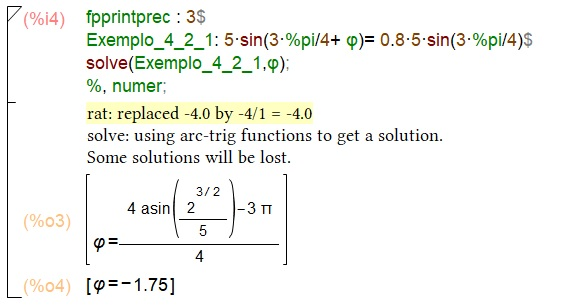
\includegraphics[width=0.7\linewidth]{exemplo421-sol}
	\label{fig:exemplo421-sol}
\end{figure}

\chapter{SIMULAÇÕES COM O MAXIMA}

\chapter{DICAS SOBRE O MAXIMA}

\begin{itemize}
	\item Se seu cálculo está demorando de mais para executar, você pode tentar os menus 'Maxima->Interromper' ou 'Maxima->Reiniciar o Maxima'.
	\item Para fazer gráficos em coordenadas polares, selecione 'Polar' em Opções na janela de gráficos bidimensionais. Você também pode fazer gráficos em coordenadas esféricas e cilíndricas em 3D.
	\item As janelas do wxMaxima têm valores padrão para as entradas, um dos quais é '\%'. Se você selecionou algo no documento, a seleção será usada no lugar de '\%'.
	\item Ao aplicar funções com um argumento a partir dos menus, o argumento padrão é '\%'. Para aplicar a função a um outro valor, selecione-o do documento antes de executar o comando do menu.
	\item Para salvar o tamanho e posição da janela do wxMaxima entre sessões, use a janela 'Maxima->Configurações'.
	\item Você pode acessar a última saída com a variável '\%'. Você pode acessar a saída de comandos anteriores usando a variável '\%on' onde n é o número da saída.
	\item Células de título, seção e subseção podem ser recolhidas para ocultar seu conteúdo. Para recolher ou expandir, clique no quadrado próximo à celula. Se você segurar Shift enquanto clica, todos os subníveis daquela célula também serão recolhidos/expandidos.
	\item Você pode esconder a saída das células clicando no triângulo no lado esquerdo das células. Isso funciona também em células de texto.
	\item Um 'cursor horizontal' foi introduzido no wxMaxima 0.8.0. Ele é mostrado como uma linha horizontal entre células. Ele mostra onde uma nova célula vai aparecer se você digitar ou colar texto, ou se executar um comando do menu.
	\item O cursor horizontal funciona como um cursor normal, mas ele opera em células: pressione as setas para cima ou para baixo para movê-lo; segure Shift enquanto move para selecionar células; pressione Backspace ou Delete duas vezes apaga a célula próxima ao cursor.
	\item Você pode selecionar vários células com o mouse - clique e arraste desde algum ponto entre células ou dos marcadores à esquerda - ou com o teclado - segure Shift enquanto move o cursor horizontal - e então operar na seleção. Isso é útil quando você quer apagar ou calcular múltiplas células.
	\item Você pode avaliar todo o documento usando o menu 'Célula->Avaliar todas as células' ou a tecla de atalho correspondente. As células serão avalidas na ordem em que aparecem no documento.
	\item As janelas do wxMaxima têm valores padrão para as entradas, um dos quais é '\%'. Se você selecionou algo no documento, a seleção será usada no lugar de '\%'.
	\item Equations have several advantages over functions. For example they can be manipulated with factor(), expand() and similar functions. They can easily be introduced one into another. Also they are always printed out as 2D maths.
	\item In text cells bullet lists can be created by beginning a line with " * ". The number of spaces in front of the "*" determines the indentation level; Indentation can be continued in the next line by indenting the line using spaces.
	\item The key combination Shift+Space results in a non-breakable space.
	\item A plot to be embedded into the work sheet by preceding its name with a "wx". "draw" can be replaced by "wxdraw", plot by "wxplot" etc.
\end{itemize}
\section{Dicas de Maxima}
Maxima's strengths are manipulating equations and in symbolic calculations. It therefore makes sense to use functions (as opposed to equations with labels) sparingly and to keep the actual values of variables in a list, instead of directly assigning them values. An example session that does do so would be:
\begin{verbatim}
/* We keep the actual values in a list so we can use them later on */
    Values:[a=10,c=100];
    Pyth:a^2+b^2=c^2;
    solve(%,b);
    result:%[2];
    at(result,Values);
    float(%);
\end{verbatim}
Maxima's "at" function allows to access to arbitrary variables in a list of results:
\begin{verbatim}
    g1:a*x+y=0;
    g2:b*y+x*x=1;
    solve([g1,g2],[a,b]);
    %[1];
    result_b:b=at(b,%);
\end{verbatim}

The "at" function allows to introduce one equation into another:
\begin{verbatim}
    ohm:U=R*I;
    r_parallel:R=R_1*R_2/(R_1+R_2);
    result:at(ohm,r_parallel);
\end{verbatim}
%%%%
The rhs() ("right hand side") command allows to retrieve the result of an equation in exactly the format a function would have:
\begin{verbatim}
    Values:[
        /* m=1.2 tons */
        m=1.2*10^3,
        /* 100 km/h*/
        v=100*10^3/(60*60)
    ];
    Energy:W=1/2*m*v^2;
    at(Energy,Values);
    W_mech:rhs(%);
\end{verbatim}
%%%%		
\end{document}
